\documentclass{projetofinal-dcc}
%%%%%%%%%%%%%%%%%%%%%%%%%%%%%%%%%%%%%%%%%%%%%%%%%%%%%%%%%%%%
%P A C O T E S
%%%%%%%%%%%%%%%%%%%%%%%%%%%%%%%%%%%%%%%%%%%%%%%%%%%%%%%%%%%%
% Adicione aqui seus pacotes

%Adicionei esse pacote pois melhora a qualidade dos espaçamentos, sem efeitos colaterais no layout do template. -- Vitor Machado
\usepackage[activate={true,nocompatibility},final,tracking=true,kerning=true]{microtype}
%Para checks e cross na tabela de comparação de frameworks de recomendação
\usepackage{pifont}% http://ctan.org/pkg/pifont
\newcommand{\cmark}{\ding{51}}%
\newcommand{\xmark}{\ding{55}}%

\usepackage[alf]{abntex2cite}
\usepackage{xspace}
\newcommand*{\eg}{\textit{e.g.}\@\xspace}
\newcommand*{\ie}{\textit{i.e.}\@\xspace}

\usepackage{multirow}
\usepackage{float}
\usepackage{booktabs}
\usepackage{lscape}
\usepackage{pdfpages}

\usepackage{breakurl}
\def\UrlBreaks{\do\/\do-}

\usepackage{tikz-uml}
\definecolor{light-gray}{gray}{0.95}

% INICIO DO DOCUMENTO
\begin{document}

% título da tese é obrigatório
\title{WppScrapper: Uma ferramenta para a extração de mensagens do WhatsApp}

% autor é obrigatório; máximo de 3 autores
\author{Lucas Ribeiro Ferreira}{Gostaria de agradecer primeiramente aos principais responsáveis pela minha formação acadêmica e pessoal. Àqueles que fizeram sacrifícios pessoais para poder prover os recursos necessários a minha educação desde meu nascimento até os dias atuais. Àqueles que me proveram tudo o que me era necessário para que eu pudesse focar em minha formação intelectual, que me proveram alicerce emocional e material durante toda a minha vida. Aos que moldaram meu caráter e estiveram presente sempre que precisei, meus pais, Eloecy e Joaquim. 

Apesar de os principais, não apenas eles foram determinantes. Então gostaria de estender esses agradecimentos aos que forneceram os alicerces necessários a esses responsáveis pelo meu. Forneceram a base de toda a família Ribeiro e a família Ferreira, que em momentos diferentes estiveram presentes de formas diferentes, porém foram todos, a sua maneira, determinantes para que eu pudesse estar entregando meu trabalho de conclusão de curso. Então meu agradecimento especial aos meus avós maternos, Lecy e Eloy e meus avós paternos, Benita e Armando.

Em decorrência de acontecimentos recentes, gostaria de fazer um agradecimento especial a minha avó Benita, que faleceu no inicio do ano em decorrência da crise pandêmica e política vivida em nosso país. Minha querida avó sempre foi especialmente carinhosa comigo e é um bom exemplo de como cada pessoa de minha família foi determinante em minha formação. Obrigado minha queria avó por ter estado comigo no intervalo entre a escola e o pré-vestibular, me fornecendo um almoço delicioso e repleto do seu amor e em outras infinidades de momentos.

Estendo ainda meus agradecimento a Beatriz, minha queria esposa, que conheci nos corredores da universidade e desde então tem sido minha companheira na jornada da vida, tornando-a mais alegre, mais amável e mais divertida. Beatriz foi fundamental ao fazer a cobrança na medida certa para que eu me dedicasse ao trabalho que estou entregando. Obrigado Bia por dividir essa vida comigo e me amar da forma que me ama, a você só posso garantir a reciprocidade de cada sentimento.

Dentre a infinidade de pessoas que atravessaram a minha vida me fornecendo ensinamentos valiosos, ajudas necessárias e companheirismo, gostaria de destacar e agradecer a minha amiga Letícia, que muito me ensinou e ensina ainda hoje, inclusive ajudando em revisões pontuais desse texto. Dentre essas pessoas também gostaria de agradecer aos meus amigos que me forneceram oportunidades de trabalho e de aprendizado profissional e pessoal Guilherme, André e Higor, estendendo a cada colega e amigo que fiz trabalhado para e com eles.

Agradeço ainda ao corpo docente da Universidade Federal Rural do Rio de Janeiro, profissionais dedicados que se esforçam para entregar um ensino de altíssima qualidade aos seus alunos. Um agradecimento especial ao professor Filipe Braida, que me orientou no curso desse trabalho com a devida paciência e cobrança, além de ter me inspirado com a dedicação que demonstrou nas aulas que ministrou ao decorrer da minha formação.

Apesar de desejar agradecer nominalmente a muitas outras pessoas, encerro agradecendo a todos aqueles que no passado lutaram e que ainda lutam para que eu pudesse ter acesso a uma universidade gratuita de qualidade e a toda a sociedade brasileira, que financiou meus estudos. Obrigado pelo investimento feito em mim e em meus colegas, me comprometo a retribuir.
}
\author{Wilson de Oliveira Mendonça}{Primeiramente gostaria de agradecer aos meus pais Heraldo e Zilma por sempre terem me dado apoio em tudo que fiz desde que nasci, por terem feito sacrifícios para me dar condições necessárias para estudar. São sem duvidas os principais responsáveis pela minha formação pessoal e acadêmica e são meus maiores exemplos.

Gostaria de agradecer ao corpo de docentes do curso de ciência da computação da Universidade Federal Rural do Rio de Janeiro por proporcionar um excelente curso, em especial ao professor Filipe Braida por todo suporte, compreensão e paciência.

Gostaria de agradecer também ao meu colega Lucas Ferreira por toda a ajuda que me deu e pela dedicação a este trabalho.}
%\author{Nome completo aluno 2}{\input{elementos-pretextuais/agradecimentos}}
%\author{Nome completo aluno 3}{\input{elementos-pretextuais/agradecimentos}}

% orientador é obrigatório
\advisor[Prof.]{Filipe Braida do Carmo,~D.Sc.}{}

% co-orientador é opcional
% \coadvisor[Prof.]{Nome do co-orientador,~M.Sc.}{}

% máximo de 3 integrantes da banca (orientador e co-orientador já são adicionados automaticamente)
\banca[Prof.]{Bruno José Dembogurski,~D.Sc.}{}
\banca[Profª.]{Natália Chaves Lessa Schots,~D.Sc.}{}
%\banca[Prof.]{Nome do participante banca 3,~Ph.D.}{COPPE~-~UFRJ}

\location{Nova~Iguaçu}{RJ}{Brasil}

% mês e ano de defesa
\date{Maio}{2021}
\maketitle

\startdocument

\includepdf[pages={2}]{folha_de_assinaturas.pdf}

% AGRADECIMENTOS
\makethankspage

% RESUMO
\begin{abstract}{
  
O WhatsApp é o aplicativo de troca de mensagens instantâneas mais utilizado no Brasil. Seu principal uso é de cunho privado entre os usuários, mas estudos recentes vêm mostrando o aumento de importância da plataforma como fonte de informação, incluindo desinformação, e como ferramenta para organização e agitação de eventos de grande relevância social, como greves e protestos. Nesse contexto, vem sendo demonstrado a importância de estudar as mensagens trocadas dentro da plataforma e, através desses estudos, ajudar a compreender as diferentes determinações da realidade social. Muitos trabalhos têm realizado a tarefa de extração de mensagens da plataforma fazendo uso de técnicas de \textit{WebScrapping} ou até descriptografando as mensagens contidas no banco de dados de um \textit{smarthphone}. Desta forma, o presente trabalho busca colaborar com essa tarefa apresentando uma ferramenta que é capaz de se conectar ao servidor do WhatsApp e baixar todas as mensagens trocadas por uma conta, possuindo uma interface de programação simples e objetiva que permite seu uso para a implementação de diferentes formas de interfaces de usuário, sendo agnóstica a qualquer que seja essa forma. Ainda é apresentado aqui uma aplicação com interface gráfica de usuário para computadores domésticos, implementada usando a \textit{API} citada anteriormente, que se propõe se de fácil uso para auxiliar pesquisadores e jornalistas a realizarem seus trabalhos mais facilmente. O objetivo que se espera alcançar com essas ferramentas é que mais estudos sejam feitos e, portanto, que possam compreender melhor nossa sociedade.


% Desta forma, o presente trabalho busca colaborar com essa tarefa apresentando uma ferramenta que é capaz de se conectar ao servidor do WhatsApp e baixar todas as mensagens trocadas por uma conta. Essa ferramenta foi escrita para que pudesse ser implementada diferentes formas de interface para a mesma. O presenta trabalho ainda apresenta uma aplicação de interface gráfica que se propõe de fácil uso para auxiliar que pesquisadores e jornalistas possam realizar seus trabalhos mais facilmente. O objetivo que se espera alcançar com essa ferramenta é que mais estudos sejam feitos e, portanto, que possam compreender melhor nossa sociedade.





}
\end{abstract}

% ABSTRACT
\begin{englishabstract}{
  WhatsApp is the most used instant messaging application in Brazil. Its main use is private among users, but recent studies have shown the increasing importance of the platform as a source of information, including misinformation, and as a tool for organizing and agitating great social relevance events, such as strikes and protests. In this context, it has been demonstrated the importance of studying the messages exchanged within the platform and, through these studies, helping to understand the different determinations of social reality. Many works have performed the task of extracting messages from the platform using WebScrapping techniques or even decrypting the messages contained in a Smartphone database. In this way, the present work seeks to collaborate with this task by presenting a tool that can connect to the WhatsApp server and download all messages exchanged by an account, it has a simple and objective programming interface that allows its use for the implementation of different forms of user interfaces, being agnostic to any form. An application with a graphical user interface for home computers is also presented here, implemented using the \textit{API} mentioned above, which is easy to use to help researchers and journalists to carry out their work more easily. The goal that is expected to be achieved with these tools is that more studies are done and, therefore, that they can better understand our society. 

% O WhatsApp é o aplicativo de troca mensagens instantâneas mais utilizado no Brasil. Seu principal uso é de cunho privado entre os usuários, mas estudos recentes vêm mostrando o aumento de importância da plataforma como fonte de informação, incluindo desinformação, e como ferramenta para organização e agitação de eventos de grande relevância social, como greves e protestos. Nesse contexto, vem sendo demonstrado a importância de estudar as mensagens trocadas dentro da plataforma e, através desses estudos, ajudar a compreender as diferentes determinações da realidade social. Muitos trabalhos têm realizado a tarefa de extração de mensagens da plataforma fazendo uso de técnicas de \textit{WebScrapping} ou até descriptografando as mensagens contidas no banco de dados de um \textit{Smarthphone}. Desta forma, o presente trabalho busca colaborar com essa tarefa apresentando uma ferramenta que é capaz de se conectar ao servidor do WhatsApp e baixar todas as mensagens trocadas por uma conta, possui uma interface de programação simples e objetiva que permite seu uso para a implementação de diferentes formas de interfaces de usuário, sendo agnóstica a qualquer que seja essa forma. Ainda é apresentado aqui uma aplicação com interface gráfica de usuário para computadores domésticos, implementada usando a \textit{API} citada anteriormente, que se propõe de fácil uso para auxiliar que pesquisadores e jornalistas possam realizar seus trabalhos mais facilmente. O objetivo que se espera alcançar com essas ferramentas é que mais estudos sejam feitos e, portanto, que possam compreender melhor nossa sociedade.

}
\end{englishabstract}

% LISTAS
%% Figuras
\makefigurespage

%% Tabelas
\maketablespage

%% Algoritmos
% \makelistingspage

%% Abreviaturas (devem estar em ordem alfabética)
% \makeabrevpage{% \item [SR] Sistema de Recomendação
% \item [CARS] Context Aware Recommender System
% \item [CDRS] Context-Driven Recommender System
% \item [JIT] Just in time
% \item [GC] Garbage Collector
% \item [LLVM] The LLVM Compiler Infrastructure
% \item [DSL] Domain Specific Language

\item [KDD] Knowledge Discovery in Databases
}

%% Símbolos (devem estar em ordem alfabética)
% \makesymbolspage{%% não está sendo usado}

% Sumário
\maketocpage

% Capítulos
\startcontent
\chapter{Introdução}

WhatsApp\footnote{https://www.whatsapp.com} é um serviço de troca de mensagens instantâneas, sendo o aplicativo de dispositivos móveis de sua categoria mais instalado no mundo \cite{sevitt2018}. A população que o utiliza com mais frequência no mundo é a população brasileira \cite{newman2019reuters}. Cerca de $53\%$ dos brasileiros utiliza o aplicativo de forma massiva para consumo de noticias, o que torna a torna mais vulnerável a propagação de desinformação \cite{newman2019reuters}.

\citeonline{marfianto2018whatsapp} afirmam que muitas pessoas utilizam da rede para crimes digitais como fraudes, redes de drogas e pornografia. \citeonline{machado2019study} demonstraram que 13\% das mensagens trocadas em grupos públicos de cunho politico na rede social durante o período da campanha eleitoral de 2018 no Brasil difundiam informações falsas. Das mensagens que possuem \textit{link} para vídeos do \textit{Youtube}\footnote{www.youtube.com}, 31\% foram consideradas desinformação.

% \citeonline{garimella2018whatapp} enfatizam a importância de que sejam feitos estudos usando as mensagens trocas em grupos públicos dentro da rede social. \citeonline{machado2019study} demonstraram que 13\% das mensagens trocadas em grupos públicos de cunho politico na rede social durante o período da campanha eleitoral de 2018 no Brasil difundiam informações falsas. Das mensagens que levavam ao \textit{Youtube}\footnote{www.youtube.com} 31\% foram consideradas desinformação. \citeonline{marfianto2018whatsapp} afirmam ainda que muitas pessoas utilizam da rede para crimes digitais como fraudes, redes de drogas e pornografia.  

Esses e outros diversos trabalhos acadêmicos e jornalísticos enfatizam a cada dia a importância da rede social no dia a dia do cidadão moderno. A rede social também tem sido usada para organização de protestos \cite{tardaguila2019epoca, resende2018system}, propaganda partidária \cite{machado2019study} e diversos outros temas \cite{garimella2018whatapp}.

\citeonline{garimella2018whatapp} defendem a importância de que sejam feitos estudos usando as mensagens trocadas em grupos públicos dentro do WhatsApp afirmando que merecem a mesma atenção que outras redes sociais. Para que esses estudos possam ser realizados, é necessária a extração das mensagens de dentro da plataforma. Contudo, o WhatsApp, devido a suas politicas de privacidade, não provê uma \textit{API} oficial para uso de pesquisadores, como outras redes sociais, \textit{e.g.} \textit{Twitter}. Na intenção de contornar essa questão, trabalhos acadêmicos foram feitos apresentando metodologias para a coleta dessas mensagens \cite{garimella2018whatapp, resende2018system}. No entanto, para fazer uso dessas metodologias se faz necessário o conhecimento de programação.

Visando facilitar o trabalho de estudar as mensagens trocadas através do WhatsApp, o presente trabalho propõe duas ferramentas análogas, mas com distintas interfaces. A primeira consiste numa interface de programação que seja capaz de extrair todas as mensagens de uma conta de WhatsApp enquanto expõe uma interface simples, coesa e objetiva. Com essa API espera-se que outros trabalhos e projetos sejam realizados usando-a para criação de programas com diferentes tipos de interface, estudos usando os dados extraídos ou melhorando a própria API. A segunda ferramenta consiste numa aplicação com interface gráfica de usuário desenvolvida para os sistemas operacionais de computadores domésticos usando a API aqui proposta nesse trabalho. Tal ferramenta poderá ser utilizada pelo usuário sem que seja exigido dele qualquer conhecimento de programação. A expectativa é que, com tal ferramenta disponível, uma quantidade maior de estudos possam ser realizados.


% , o presente trabalho se propõe a desenvolver uma ferramenta para extração dessas mensagens. Tal ferramenta deverá poder ser utilizada pelo usuário sem que seja exigido dele qualquer conhecimento de programação. A expectativa é que, com tal ferramenta disponível, uma quantidade maior de estudos possam ser realizados.

% Partindo do pressuposto que mais trabalhos que ajudem a compreender o que acontece nos grupos públicos de WhatsApp precisam ser feitos e que o conhecimento de programação pode ser um limitador para tal, o presente trabalho se propõe a desenvolver uma ferramenta para extração de mensagens de grupos públicos do WhatsApp que seja de fácil utilidade e sem o requisito de conhecimentos de programação.

O trabalho está divido em cinco capítulos, incluindo esta breve introdução do problema que se propõe a ajudar a resolver. No segundo capítulo são apresentados os conceitos de Mineração de Dados, junto a uma pequena introdução de Mineração de Texto e Mineração de Web, e \textit{Web Scraping}. No capítulo seguinte é apresentado a motivação desse trabalho seguido dos trabalhos relacionados. Nesse mesmo capítulo ainda é apresentado com mais detalhes a proposta. No quarto capítulo estão descritas as tomadas de decisão feitas para a implementação do projeto, junto com uma breve descrição das tecnologias utilizadas, e uma apresentação da aplicação desenvolvida. O quinto e último capítulo conta as conclusões do trabalho e trabalhos futuros. 
\chapter{Fundamentação}\label{chp:LABEL_CHP_2}

Esse capitulo trata da mineração de dados descrevendo os principais objetivos desse campo de estudos, suas principais técnicas e aplicabilidades. Ele também descreve a técnica de \textit{Web Scraping}.

\section{Mineração dos Dados}

% Estrutura:
% Intro a mineração de dados. Motivação e "nascimento"
% Processo de descoberta de conhecimento
% Pequena introdução ao CRISP.
% Preparação de dados
% As técnicas da mineração de dados
% Os tipos de método da mineração de dados
% Exemplo de algoritmo relacionando com uma técninca e um tipo de método
% Chamar atenção para que pesquisadores criam dados para estudar por não ter acesso a eles.
% Estabelecer que uma das limitações é o formato de entrada
% Introduzir a mineração de texto
% Introduzir mineração de mídias sociais
% Introduzir mineração de dados. Definição, problema que motiva.

Tradicionalmente, para extrair conhecimento de dados, é necessária uma análise e interpretação manual dos mesmos \cite{fayyad1996data}. \citeonline{fayyad1996data} exemplificam dizendo que é comum que, na área de saúde, sejam gerados relatórios periódicos feitos por especialistas por meio da análise dos dados do plano de saúde e que, com base nesses relatórios, são feitos os planejamentos gerenciais e futuras tomadas de decisão.

Porém, com o volume de dados crescendo drasticamente, esse método de análise está se tornando impraticável para muitos domínios. Mesmo quando é possível realizar a análise, esse processo pode ser lento, caro e muito subjetivo \cite{fayyad1996data}. Empresas gastam milhões de reais para coletar e armazenar dados sem que informações uteis possam ser identificadas \cite{camilo2009mineraccao}. Foi com o intuito de solucionar esse problema que, no final da década de 80, foi proposta a Mineração de Dados \cite{camilo2009mineraccao}.

Alguns autores tratam a Descoberta de Conhecimento nas Bases de Dados (\textit{Knowledge Discovery in Databases} - KDD) como sinônimo de Mineração de dados, enquanto outros tratam a Mineração de Dados como uma parte do processo de KDD \cite{camilo2009mineraccao}. Para \citeonline[p.~40-41, tradução nossa]{fayyad1996data}, KDD é "um processo não trivial de identificação de novos padrões válidos, úteis e compreensíveis". \citeonline{cortes2002mineraccao} definem Mineração de Dados como:

\begin{quote}
    (...) um processo altamente cooperativo entre homens e máquinas, que visa a exploração de grandes bancos de dados, com o objetivo de extrair conhecimentos através do reconhecimento de padrões e relacionamento entre variáveis, conhecimentos esses que possam ser obtidos por técnicas comprovadamente confiáveis e validados pela sua expressividade estatística \cite[p.~1-2]{cortes2002mineraccao}.
\end{quote}

O processo de mineração é iterativo, interativo e dividido em fases \cite{camilo2009mineraccao}. \citeonline{fayyad1996data} separa o processo de \textit{KDD} em seleção, pré-processamento, transformação, mineração de dados e interpretação/avaliação, ilustrado na figura \ref{fig:kdd-geral}.

\begin{figure}[h!]
    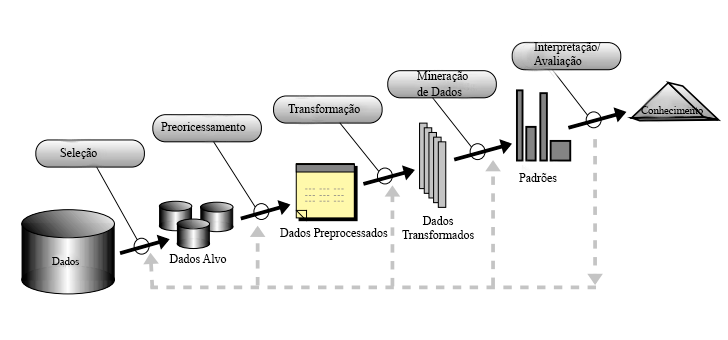
\includegraphics[width=\textwidth]{img/kdd.png}
    \caption{Uma visão geral dos passos que compõem um processo KDD. Adaptado de \citeonline{fayyad1996data}}
    \centering
    \label{fig:kdd-geral}
\end{figure}

O processo CRISP-DM (\textit{Cross-Industry Standard Processo of Data Mining}), que pode ser considerado o de maior aceitação hoje em dia \cite{camilo2009mineraccao}, é dividido em seis fases, apresentadas na figura \ref{fig:crisp}: entendimento do negócio, entendimento dos dados, preparação dos dados, modelagem, avaliação e implantação \cite{olson2008advanced}.

\begin{figure}[h]
\centering
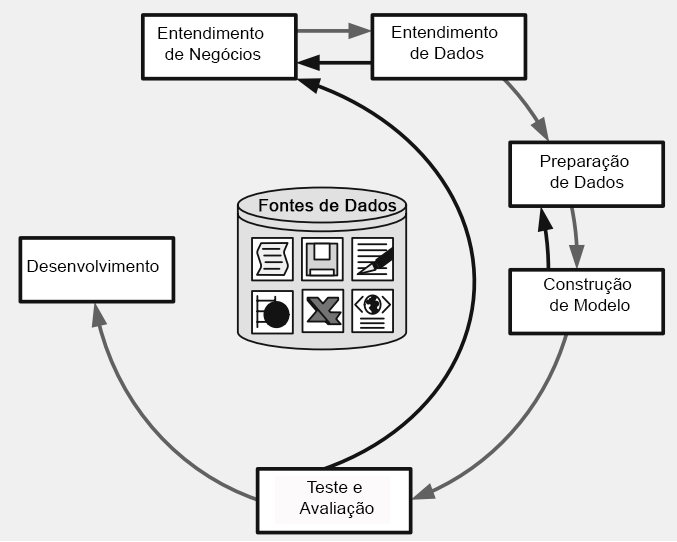
\includegraphics[width=0.8\textwidth]{img/crisp.png}
\caption{Processo CRISP-DM. Adaptado de \citeonline{olson2008advanced}}
\label{fig:crisp}
\end{figure}


Os dados podem ser qualitativos ou quantitativos. O primeiro são dados com valores nominais e categóricos. Já o segundo, diz respeito a dados com valores numérico, sejam eles discretos ou contínuos \cite{camilo2009mineraccao}. Para escolher o método a ser utilizado, é fundamental entender qual o tipo do dados será utilizado como entrada, e para utilizá-los, geralmente é preciso prepará-los \cite{camilo2009mineraccao}. \citeonline{camilo2009mineraccao} ressaltam:

\begin{quote}
    Devido às diversas origens possíveis, é comum que os dados não estejam preparados para que os métodos de Mineração de Dados sejam aplicados diretamente. Dependendo da qualidade desses dados, algumas ações podem ser necessárias. Este processo de limpeza dos dados geralmente envolve filtrar, combinar e preencher valores vazios
    \cite[p.~4]{camilo2009mineraccao}.
\end{quote}

A fase de preparação dos dados pode ocupar, sozinha, a maior parte do processo \cite{camilo2009mineraccao}. Para melhor entender os dados de forma a auxiliar na escolha de como prepará-los, são utilizados diversas técnicas de visualização de dados \cite{camilo2009mineraccao}. Após obtido conhecimento sobre dados, é possível escolher a melhor forma de prepará-lo para a mineração. Na preparação se realiza a limpeza de dados, integração de dados, transformação dos dados e redução dos dados \cite{han2011data}.

Muita vezes, quando se cria um modelo para um conjunto de dados de um problema, ele não se mostra satisfatório para um outro conjunto de dados do mesmo problema. Isso se dá pois o modelo se torna enviesado aos dados com os quais ele foi treinado. Esse efeito é conhecido como efeito \textit{Bias}. Para evitar isso, normalmente se divide o conjunto em três partes: conjunto de treinamento, conjunto de testes e conjunto de validação \cite{camilo2009mineraccao}.

\citeonline{camilo2009mineraccao} ressaltam que, apesar da existência massiva de dados sob posse das empresas, normalmente esses dados não são disponibilizados para pesquisadores. Devido a isso é comum se criar algoritmos teóricos e validá-los com dados sintéticos. Desta forma, não tendo a possibilidade de testá-los em um ambiente real.

A mineração de dados possui dois principais objetivos: predição e classificação. A predição consiste em usar parte dos dados ou dos campos para inferir valores de outros campos ou valores futuros dos mesmos. A classificação foca em encontrar padrões descritivos que humanos possam interpretar \cite{fayyad1996data}. 

Existem diversas técnicas para auxiliar a alcançar os objetivos. Dentre elas estão: classificação, regressão, descrição, agrupamento, associação e predição \cite{fayyad1996data}. Cada uma dessas técnicas possuem diversos métodos e algoritmos, que podem ser supervisionados, não-supervisionados ou uma variação entre os dois \cite{camilo2009mineraccao}.

Regressão Linear, por exemplo, é um método supervisionado de predição, que objetiva encontrar um possível valor futuro para uma variável. O método consiste em encontrar uma função linear a partir dos dados existentes onde o valor de \textit{y} é estimado em função de uma variável \textit{x} \cite{camilo2009mineraccao}.

\begin{figure}[h]
\centering
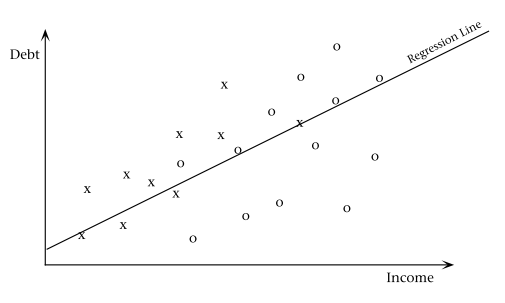
\includegraphics[width=0.8\textwidth]{img/linear-reg.png}
\caption{Uma regressão linear simples de um conjunto de dados de empréstimo. Adaptado de \citeonline{fayyad1996data}}
\label{fig:linear-reg}
\end{figure}

Uma das limitações da mineração de dados está no formato do dado de entrada. Inicialmente pensadas para serem aplicadas em dados estruturados em bancos de dados ou arquivos, as técnicas de mineração podem não ter mesma eficácia ao lidar com dados em outros formatos, \textit{e.g.} multimídia, texto, espacial. Devido a isso muitos estudos tratando a mineração de dados complexos vem sendo feitos \cite{camilo2009mineraccao}. Um exemplo disso é a mineração de textos.

Devido à falta de estrutura, dados textuais normalmente são manipulados por meio de motores de busca, diferente de dados estruturados, que normalmente são manipulados por meio de sistemas de banco de dados. Motores de busca são eficientes no objetivo de levar o usuário à informação correta no tempo correto, mas a mineração de texto é mais que isso. Mineração de texto pode ajudar o usuário a digerir a informação e ajudar na tomada de decisão \cite{aggarwal2012mining}. \citeonline{aggarwal2012mining} completam:

\begin{quote}
    Existem diversas aplicações para a mineração de texto onde o objetivo primário é analisar e descobrir algum padrão interessante, incluindo tendencias e \textit{outliers}, em dados textuais, e a noção de busca não é essencial ou mesmo relevante \cite[p.~2, tradução nossa]{aggarwal2012mining}.
    % Text mining can be regarded as go- ing beyond information access to further help users analyze and digest information and facilitate decision making.There are also many applica- tions of text mining where the primary goal is to analyze and discover any interesting pattterns, including trends and outliers, in text data, and the notion of a query is not essential or even relevant.
\end{quote}

\citeonline{marfianto2018whatsapp} apresentam o que pode ser usado com um exemplo de uso de mineração de texto. O trabalho utiliza de técnicas de mineração de texto para fazer uma análise forense das mensagens do WhatsApp de um suspeito com o intuito de ajudar a extrair evidências criminalísticas.

% [
% \textbf{Preciso de um jeito de fazer uma ponte entre mineração de texto e mineração de opinião e mineração de redes sociais.
% Essa ponte é feita no livro \cite{aggarwal2012mining}, mas não consigui pensar num jeito de fazer de forma enxuta e rápida.}
% ]

Uma das fontes de texto mais comuns são as redes sociais. Elas permitem que as pessoas se expressem de forma rápida e livre em contextos muito abrangentes. Para minerar texto dessas fontes é necessário técnicas específicas, pois podem conter um vocabulário coloquial e sem padronização. Métodos que fazem uso tanto das conexões da rede social quanto do conteúdo, por exemplo, conseguem prover resultados mais eficientes que os que usam apenas o conteúdo ou conexões \cite{aggarwal2012mining}. 

As formas mais comuns de mineração de conteúdo da internet é feito através de mineração de dados não-estruturados, mineração de dados estruturados, mineração de dados semi-estruturados ou mineração de dados multimídia. A coleta de dados para mineração é uma tarefa importante para a mineração de dados não-estruturados e um dos maiores desafios, devido à complexidade de todas as \textit{tags} \textit{HTML} que podem estar presentes. \textit{Web Scrapers} ajudam a simplificar essa tarefa \cite{dastidar2016intelligent}.

% The major forms of web content mining are done in the following ways:
% ? Unstructured data mining ? Structured data mining ? Semi-structured data mining

% Under the subtopic of unstructured data mining comes the mining of web documents which this paper deals with. Personal Information retrieval is a challenging task when it comes to mining from web pages, primarily because of the complexity of all the HTML tags that may be present. Web scrapers help a great deal in simplifying the task.


% Exemplificar mineração de dados com os diferentes tipos

\section{\textit{Web Scraping}}

A internet se tornou a maior fonte de dados do mundo \cite{banerjee2014website}. A geração de dados e o crescimento de sua taxa está aumentando a cada dia \cite{dastidar2016intelligent}. A internet foi projetada para que seja fácil para que pessoas encontrem informações \cite{banerjee2014website}. Usuários na internet podem usufruir abundantemente de serviços e informação, \textit{e.g.} comércio eletrônico, \textit{websites}, jornais eletrônicos, redes sociais e blog \cite{dastidar2016intelligent}. Mas, se a única forma de acessar esses dados for por meio de um navegador \textit{web}, uma grande variedade de possibilidades será perdida \cite{mitchell2018web}. 

Muitas empresas, com o objetivo de localizar, capturar e guardar um enorme volume de informação que precisam de \textit{websites}, ainda usam de métodos tradicionais de extração de dados da internet, como o manual "copia e cola" \cite{banerjee2014website}. O processo de extração manual consiste na empresa contratar uma grande quantidade de funcionários e orientá-los a fazer a extração navegando pelas páginas copiando os dados para um banco de dados \cite{banerjee2014website}. Tal processo, além de muito caro, também é muito suscetível a erros humanos \cite{banerjee2014website}. 

Outra possibilidade para recuperar essas informações seria por meio das APIs (\textit{Application Program Interface}). Uma \textit{API} define uma sintaxe padronizada que permite uma parte de um software se comunicar com uma outra parte, mesmo que eles tenham sido escritos em linguagens diferentes ou estruturados de forma diferente \cite{mitchell2018web}. É possível encontrar \textit{APIs} de diversos tipos de dados que podem ser utilizados, \textit{e.g}. postagens do \textit{Twitter}\footnote{www.twitter.com}, paginas do \textit{Wikipedia}\footnote{www.wikipedia.com}. Apesar de ser preferível fazer uso das APIs, elas podem não existir para o dado desejado ou possuir limitações de acesso, \textit{e.g} quantidade de acessos por dia \cite{mitchell2018web}.

Páginas HTML é a principal ferramenta de formação de informação na internet. \citeonline[p.~25]{dastidar2016intelligent} define \textit{Web Scraping} como o processo de extrair informações úteis dessas paginas usando qualquer linguagem de programação. Para \citeonline{mitchell2018web}, é na prática uma vasta variedade de técnicas de programação e tecnologias, como análise de dados, análise de linguagem natural e segurança da informação. \citeonline{mitchell2018web} ainda define teoricamente como:

\begin{quote}
    (...) a prática de recuperar dados por meio de qualquer outro meio que não um programa interagindo com uma API (ou, obviamente, por meio de um humano usando um navegador). Normalmente, isso é alcançado escrevendo um programa automatizado que consulta um servidor \textit{web}, requisita dados (normalmente em forma de HTML e outros arquivos que compõem uma página \textit{web}), e então analisa esses dados pra extrair a informação necessária
    \cite[p.~ix, tradução nossa]{mitchell2018web}.
    % is the practice of gathering data through any means other than a program interacting with an API (or, obviously, through a human using a web browser). This is most commonly accomplished by writing an automated program that queries a web server, requests data (usually in the form of HTML and other files that compose web pages), and then parses that data to extract needed information.
\end{quote}

Uma das aplicabilidades da técnica de \textit{Web Scraping} é na mineração de dados na internet \cite{dastidar2016intelligent}. Mineração de internet, como explica \citeonline[p.~197-198, tradução nossa]{shi2009web}, "é uma área de pesquisa que tenta identificar pedaços de informação aplicando técnicas de mineração de dados e aprendizado de máquina a documentos e dados da internet". As principais formas de mineração de conteúdo na internet é feito por meio de mineração de dados não-estruturados, mineração de dados estruturados, mineração de dados semi-estruturados e mineração de dados multimídia \cite{dastidar2016intelligent}.

Devido à complexidade das \textit{tags} \textit{HTML}, recuperar informações de documentos na internet pode se tornar uma tarefa complicada, mesmo sendo uma parte importante da mineração de dados não-estruturados. \textit{Web Scraping} simplifica significativamente essa tarefa \cite{dastidar2016intelligent}.

Um exemplo de uso de \textit{Web Scrapping} pode ser encontrado no trabalho de \citeonline{boeing2017new}. Os autores extraíram a listagem de aluguéis de casas nos Estados Unidos do site \textit{Craiglist}\footnote{http://craigslist.org/} e conseguiram demonstrar novas informações sobre padrões de distribuição espacial do mercado de casas no país de forma mais rica que utilizando outras fontes de informações públicas, como o censo.
\chapter{Coletor de Dados para WhatsApp}

Esse capitulo apresenta as motivações do presente trabalho, seguido pelos trabalhos relacionados e a descrição da aplicação proposta.

\section{Motivação}

Com a facilidade de trocar mensagens e criar grupos de forma gratuita por meio de aplicativos mensageiros, criou-se um novo meio de formação de comunidades. Essas comunidades normalmente giram em torno de um tema, que são diversos, \textit{e.g.} família, política, esportes, animes, ativismo, negócios, trocas e educação, grupos que podem ser públicos ou privados \cite{garimella2018whatapp}.

O Whatsapp é o mensageiro mais instalado no mundo \cite{sevitt2018} e a população brasileira é uma das mais assíduas nessa rede social \cite{newman2019reuters}. Cerca de $84\%$ dos brasileiros são usuários do aplicativo, que é a rede social mais popular no país, $53\%$ consomem e compartilham notícias por meio da rede \cite{newman2019reuters}. \citeonline{newman2019reuters} também chamam atenção que no Brasil os usuários de Whatsapp fazem parte de grupos com pessoas que não conhecem com mais frequência que nos países ocidentais, associando isso ao uso da ferramenta como uma fonte de notícias, informação e facilitando a propagação de desinformação.

Há alguns anos esses grupos de Whatsapp vem desempenhando um papel importante na sociedade como uma ferramenta de mobilização de massas. Em 2018, a rede social foi primordial para a organização e agitação de uma das maiores greves de caminhoneiros do Brasil. Cerca de $45\%$ dos caminhoneiros tiveram conhecimento da manifestação por meio do aplicativo \cite{deotti2018ipsol}. Esse mesmo evento pôde ser monitorado pelo sistema de monitoramento de grupos públicos de WhatsApp apresentado por \citeonline{resende2018system}, o que reforça a importância da rede na mobilização, como reportado por \citeonline{amanda2018bbc}.

De semelhante modo, os grupos de WhatsApp estão sendo utilizados para a disseminação de desinformação, com notícias falsas e discursos de ódio. Durante a campanha presidencial de 2018 no Brasil, \citeonline{machado2019study} coletaram mensagens grupos de cunho político no aplicativo e mostraram que $13\%$ das mensagens difundiam informação falsa. Das mensagens que levavam a vídeos no \textit{Youtube}\footnote{http://www.youtube.com.br}, que representam $40\%$ dos links compartilhados, $31\%$ foram consideradas desinformação e das que levavam ao \textit{Facebook}\footnote{\label{foot:facebook}http://www.facebook.com} $42\%$. Dentre todos os vídeos compartilhados pela rede $9,5\%$ correspondiam a discurso de ódio, violência extrema explícita ou pornografia atacando minorias. O estudo ainda aponta que mensagens desse último tipo frequentemente são utilizadas como estratégia para que se alcance uma disseminação viral.

Reforçando a importância da rede social na disputa eleitoral, \citeonline{machado2019study} demonstraram que $65\%$ dos vídeos compartilhados nos grupos foram classificados como favoráveis ao candidato vencedor das eleições enquanto apenas $5\%$ correspondiam a defesa do seu principal oponente na disputa. Dentre as imagens compartilhadas, a proporção foi de $58,5\%$ e $15,5\%$ respectivamente.

Estudar as interações em grupos do WhatsApp vem se mostrando uma forma eficiente de entender os acontecimentos sociais. \citeonline{garimella2018whatapp} reforçam a ideia dizendo que estudar o WhatsApp deve ter a mesma relevância que estudar outras redes sociais. Porém, coletar as mensagens trocadas na plataforma não é uma tarefa simples devido a falta de uma ferramenta específica, como é possível encontrar para outras redes sociais populares como \textit{Facebook} ou \textit{Twitter}\footnote{http://www.twitter.com}.

\citeonline{garimella2018whatapp} coletaram as mensagens acessando o banco de dados do dispositivo móvel e descriptografando-as, o que não seria possível ser feito sem conhecimentos de programação específicos. O WhatsApp possui uma plataforma Web onde os usuários podem trocar as mensagens usando o navegador. Tal plataforma foi utilizada por \citeonline{resende2018system} para contornar a criptografia ponta a ponta programando um \textit{crawler} que fica coletando as mensagens presente no HTML da página. Apesar do trabalho disponibilizar seus códigos de forma pública na internet, ainda se faz necessário ter conhecimentos de programação para poder utilizar das mesmas metodologias.

Hoje, para que pesquisadores ou jornalistas possam estudar de forma quantitativa as interações em grupos públicos de WhatsApp, é vital o conhecimento de programação. Tornar a coleta de mensagens de Whatsapp uma tarefa menos técnica, pode facilitar que profissionais de outras áreas façam mais estudos. 

% A persistência de tal requisito pode impactar negativamente, limitando a quantidade de estudos sobre a plataforma.

\section{Trabalhos Relacionados}
\label{cap:trabalhosrelacionados}

Devido ao seu protagonismo em recentes eventos pelo mundo, a quantidade de trabalhos na literatura que exploram o uso do Whatsapp tem aumentado, alguns deles propondo metodologias para extração de dados junto a uma análise \cite{resende2018system, garimella2018whatapp}. Por outro lado, outros trabalhos focam em classificar dados quantitativos de grupos públicos e analisar o comportamento desses, sem entrar em detalhes mais técnicos sobre a fase de coleta \cite{machado2019study, caetano2018analyzing}. Todos eles ressaltam a necessidade de ser fazer ainda mais estudos envolvendo o aplicativo, tanto para melhor entender como se dá o comportamento das pessoas na plataforma, como para compreender como ela vem sendo utilizada por atores da sociedade.

\citeonline{resende2018system} apresentam uma metodologia de extração de dados que se resume em três etapas: coleta de \textit{links} para grupos de Whatsapp de interesse da pesquisa, inscrição nesses grupos e coleta de mensagens e demais informações. Para a última etapa foi utilizado um \textit{crawler} \textit{web} que extrai as informações disponíveis na versão \textit{web} do Whatsapp, livre de criptografias. Também foi utilizado um \textit{script} para automatizar a primeira etapa. Tal trabalho confirmou seu valor ao ser utilizado em matérias jornalisticas como as publicadas na BBC \cite{amanda2018bbc}, G1, Folha de São Paulo e Época \cite{tardaguila2019epoca}.

\begin{quote}
    Além de descrever nossa metodologia, também fornecemos uma breve caracterização do conteúdo compartilhado por 6.314 usuários em 127 grupos públicos brasileiros do WhatsApp com temáticas relacionadas à política e notícias gerais. Nós acreditamos que nosso sistema possa ajudar jornalistas e pesquisadores a entender a repercussão de eventos relacionados às eleições brasileiras dentro desse espaço midiático.
    \cite[p.~387]{resende2018system}
\end{quote}

% O trabalho de \citeonline{resende2018system} confirmou seu valor ao ser utilizado em matérias jornalisticas como as publicadas na BBC \cite{amanda2018bbc}, G1, Folha de São Paulo e Época \cite{tardaguila2019epoca}.

De forma semelhante a \citeonline{resende2018system}, \citeonline{garimella2018whatapp} também utilizaram de um \textit{crawler} para registrar contas de Whatsapp em uma lista de grupos obtidos anteriormente. Mas, para coletar as mensagens, \citeonline{garimella2018whatapp} extraíram e descriptografaram o banco de dados acessando fisicamente o dispositivo móvel que está registrado na conta. O objetivo deste trabalho está em prover contexto aos grupos públicos de WhatsApp para que pesquisadores possam compreender quais dados podem ser coletados e como podem ser utilizados. O trabalho conclui que:

\begin{quote}
    (...) como um popular meio de comunicação em muitas partes do mundo, nós argumentamos que o WhatsApp deve receber uma atenção equivalente a outros serviços de mídia social, \textit{e.g.} Twitter. Nós esperamos que esse trabalho, e as ferramentas associadas a ele, possam servir como uma plataforma para outras pesquisas construírem sobre.
    \cite[p.~387, tradução nossa]{garimella2018whatapp}
    
    % Original - Conclusão
    % However, as a popular medium for communication inmany parts of the world, we argue that WhatsApp should begiven equal attention to that of other social media services,e.g.,Twitter. We hope that this work, and its associated tools,can act as a platform for other research to build atop of
\end{quote}

% <<Original>> Garimella 2018 - Abstract
% To provide context, we perform statistical exploration to allow researchers to understand what public WhatsApp group data can be collected and how this data can be used. Given the widespread use of WhatsApp, our techniques to obtain public data and potential applications are important for the community.

% Com o intuito de prover contexto, \citeonline{garimella2018whatapp} também "realiza uma analise estatística para permitir que pesquisadores entendam de qual publico os dados de grupos de Whatsapp podem ser coletados e como esses dados podem ser utilizados".


Em \citeonline{machado2019study} encontra-se um importante trabalho de análise sobre dados coletados do Whatsapp. Além de achados que reforçam o tom da importância da rede social nas eleições brasileiras de 2018, o estudo apresentou um método para classificação do conteúdo coletado. A classificação foi feita de acordo com a origem da informação: conteúdo profissional de notícia, profissional de política e de polarização e conspiração; e de acordo com a afinidade política. Outras conclusões do trabalho:

\begin{quote}
    (1) No Brasil, WhatsApp apresenta um nímero extremamente pequeno de conteúdo político profissional e um alto número de conteúdo enganoso; (2) A propagação da informação no WhatsApp depende de uma disseminação intensa de arquivos de mídia, que não usa a mesma retórica que fontes de notícias enganosas, não tentam simular uma autoridade para creditar a informação; (3) Estratégias de disseminação de conteúdo em grupos de WhatsApp frequentemente recorre a discurso de ódio e engano para alcançar uma disseminação viral. Nossa investigação indica que metáforas visuais estão sendo pesadamente utilizadas dentro dos grupos de WhatsApp para distorcer informação e manipular os usuários  \cite[p.~1017, tradução nossa]{machado2019study}.
    
    % (1) In Brazil, WhatsApp presents an extremely  low  number  of  professional  political  content  and  a high number of junk news content; (2) Information spreading on WhatsApp  relies  intensely  on  the  dissemination  media  files, which don’t use the same rhetoric as junk news sources, not attempting  to  simulate  authority  to  credit  information;  (3) Content dissemination strategies within WhatsApp groups often resort  to  hate  speech  and  deception  to  achieve  viral dissemination. Our investigations indicate that visual metaphors are  being  heavily  used  within  WhatsApp  groups  to  distort information and manipulate users. 
\end{quote}

Usando uma estratégia de coleta de dados semelhante à proposta por \citeonline{resende2018system}, o estudo de \citeonline{caetano2018analyzing} se caracteriza pelo o que afirma acreditar ser, na literatura científica, a primeira análise significante do comportamento de grupos no WhatsApp. O trabalho introduz um \textit{framework} e métricas para caracterizar o comportamento de grupos de comunicação em aplicativos de troca de mensagem móveis como o WhatsApp. Diferente de outros trabalho, esse não se preocupa com o conteúdo em si, mas sim com dados como a frequência de mensagens, nível de atividade de usuários em grupos, proporção de mensagens trocadas em forma de arquivo de mídia, emoji e textual, dentre outros. O estudo exemplifica a utilidade das métricas as utilizando para comparar grupos políticos a não políticos.

\begin{quote}
    Vale a pena mencionar que, apesar do cenário desse artigo ser contrastar grupos públicos políticos e não políticos de WhatsApp, nós acreditamos que nossa metodologia pode ser aplicável em diversos cenários e também em outras plataformas de mensagem instantânea. (...)
    
    Nós esperamos que os achados desse artigo possam contribuir para clarear a forma que o WhatsApp funciona e reduzir a opacidade de serviços modernos da infraestrutura global de comunicação de informação.
    \cite[p.~1013, tradução nossa]{caetano2018analyzing}.
    
    % It is worth mentioning that, despite this paper scenario is to contrast WhatsApp political and non-political public groups, we believe that our methodology is applicable to several scenarios and also to other instantaneous messaging platforms. Demonstrating this applicability is one of our fu- ture work directions, together with better understanding the role of each user in the group, as well as how it evolved across time. We also want to correlate observed behavior to external events and to assess how the impact of such events varies among groups.
    % We expect that the findings provided in this paper contribute to shed light on the way WhatsApp works and reduce the opaqueness of the modern services of the global commu- nication and information infrastructure.
\end{quote}

Todos os trabalhos citados aqui propõem metodologias de extração ou análise de dados onde, apesar de muito úteis tanto para pesquisadores quanto para jornalistas, há a necessidade de conhecimentos de programação para a realização da etapa de coleta. Seja para a implementação de um \textit{script} ou para o uso daqueles disponibilizados publicamente. O presente trabalho, diferente dos anteriores, introduz uma ferramenta de fácil instalação e uso por não programadores para a extração de mensagens e outras informações de grupos públicos de WhatsApp na tentativa de promover ainda mais dinamismo e incentivar o aumento da quantidade de pesquisas sobre a plataforma.

\section{Proposta}
\label{cap:proposta}

% Resumo do problema a ser resolvido, pequena intro
% Como meu trabalho resolve esse problema ?
% Descrever a metodologia de coleta e extração das mensagens
% Descrever a ferramenta de extração das mensagens
% Descrever a API GO de extração das mensagens que ficará disponível também.


% §1 Resumo do problema
Sua natureza privada e pessoal manteve o WhatsApp fora do foco de acadêmicos por muito tempo, com trabalhos se limitando a estudos qualitativos com uso de voluntários \cite{garimella2018whatapp}. Para manter a segurança e a privacidade de seus usuários, o aplicativo mantém suas mensagens criptografadas de ponta a ponta. Além disso, o WhatsApp não disponibiliza nenhuma forma oficial para a coleta de informações para pesquisadores, diferente do Facebook e Twitter. 

% §2 Resumo da relevância de se atacar o problema
Tendo em vista cenário apresentado, estudar o aplicativo vem se mostrando cada vez mais essencial para que se possa compreender a sociedade e os eventos que nela ocorrem. Mesmo sendo uma tarefa especialmente complexa dada a sua natureza, a quantidade de estudos sobre o WhatsApp vem crescendo e reforçam a importância de que mais trabalhos sejam feitos nessa direção. Para que esses trabalhos pudessem ser feitos, foi preciso contornar as limitações que a plataforma impõe utilizando técnicas de programação. Tal requisito pode ser um impeditivo para que outros pesquisadores façam seus trabalhos.

% §3 Resumo da ideia básica de como contornar o problema.
Com o objetivo de facilitar pesquisas sobre as interações interpessoais dentro dos grupos públicos de WhatsApp, o presente trabalho se propõe a disponibilizar uma ferramenta de fácil uso e livre do requisito de conhecimento programação para extração de mensagens e outras informações relevantes desses grupos. Para isso, tal ferramenta deverá contar com mecanismos de interface gráfica e poder ser usada em um computador pessoal.

% Esse parágrafo adicionei depois. Ele servirá de gancho em parágrafos mais a frente para apresentar mais detalhadamente essa API. Não faz parte da linha argumentativa principal que estou contando os parágrafos, por isso não contei esse.
O trabalho também se propõe a implementar a aplicação de forma que sua API interna seja desacoplada de seu código de interface. Sendo assim, também será disponibilizado a API em um repositório separado para que possa ser implementada as mais diversas e úteis formas de interface que se faça necessário. Tais interfaces, \textit{e.g} linha de comando, Rest, \textit{Socket}, poderão ser implementadas posteriormente por qualquer um que desejar. Dessa forma, as pessoas interessadas poderão concentrar seus esforços em implementar a interface de usuário desejada e também poderão contribuir para a melhoria da API caso haja interesse. Tal como a ferramenta de interface gráfica, a API será concentrada na extração de mensagens trocadas por uma conta de WhatsApp. 

% §4 Pq os trabalhos relacionados não são solução. 
% Falar da necessidade de uma etapa de coleta das mensagens. Onde o usuário apenas entra nos grupos usando um dispositivo móvel e deixa o mesmo ligado recebendo as mensagens. Coleta -> Extração. Preciso aqui descrever num nível mais alto de abstração como se dará a metodologia toda de coleta até a extração e comparar com os trabalhos relacionados.
No método apresentado por \citeonline{resende2018system}, foi utilizado a ferramenta \textit{WebWhatsAppAPI}\footnote{\href{https://github.com/mukulhase/WebWhatsapp-Wrapper}{https://github.com/mukulhase/WebWhatsapp-Wrapper}} para que pudesse ser feito a coleta das mensagens contornando a criptografia. Tal ferramenta, apesar de eficiente, necessita de muitas etapas de configuração de ambiente e sua manipulação é inteiramente feita via linha de comando ou via codificação de \textit{scripts}. \citeonline{garimella2018whatapp}, por sua vez, apresenta uma metodologia em que em uma etapa as mensagens são coletadas usando um \textit{smartphone}, com o WhatsApp instalado, deixando este com uma conta autenticada e devidamente inscrita nos grupos em que há interesse em coletar as mensagens. Em uma etapa posterior é usado um programa que é capaz de acessar o banco de dados do WhatsApp e fazer a descriptografia do mesmo, conectando esse \textit{smartphone} a um computador. Em face das constantes atualizações de segurança do WhatsApp, a realização dessa segunda etapa pode se tornar um impeditivo, além de também necessitar que usuário possua um conjunto de habilidades ligados à tecnologia da informação. Necessidade essa que o presente trabalho se propõe a contornar.

% §5 Como meu trabalho se diferencia do deles? Em linhas gerais, como se dará a extração usando meu método e programa?
A metodologia para a coleta e extração das mensagens proposta no presente trabalho, no nível mais alto, se assemelha ao trabalho de \citeonline{garimella2018whatapp} pois também faz uso da estratégia de duas etapas. Na primeira etapa, de coleta das mensagens, o usuário deverá configurar um dispositivo móvel com uma conta de WhatsApp e subscrever em todos os grupos que deseja coletar mensagens. Uma vez que o aplicativo estiver devidamente configurado, ele começará a receber as mensagens e guardá-las localmente em um banco de dados. Na segunda etapa, de extração das mensagens coletadas, que é onde o presente trabalho se concentra, deverá ser usada a ferramenta aqui proposta, que será capaz de extrair todas as mensagens coletadas na primeira etapa e seu uso se dará através de uma interface gráfica de usuário em um computador pessoal. Nos próximos parágrafos será descrito com mais detalhes as características, funcionalidades desse \textit{software}.

% Introdução da ferramenta
O WppScrapper GUI, ferramenta que será implementada e apresentada no próximo capítulo, tem como seu principal objetivo prover ao usuário uma interface através da qual ele será capaz de extrair todas as mensagens trocadas por uma conta de WhatsApp que ele possua. O usuário aqui idealizado é aquele que possui o interesse em extrair essas informações do WhatsApp mas não possui conhecimentos de programação requeridos para fazê-lo usando interfaces de programação ou de linha de comando disponíveis. Tendo em vista esse usuário, deve-se projetar uma ferramenta mais simples e objetiva possível e onde todo seu uso seja através da interface gráfica. Esse software deverá poder ser usado em um computador pessoal qualquer. 

% Funcionalidade relevante, que está nos trabalhos relacionados, mas que não vamos atacar.
Acreditando ser um impeditivo menor, a ferramenta a ser implementada não visa automatizar a etapa de inscrição automática nos grupos públicos de WhatsApp, nem mesmo a coleta dos links dos mesmos. Tais etapas poderão continuar sendo realizadas das formas propostas por \citeonline{resende2018system} ou \citeonline{garimella2018whatapp}, tal como qualquer outro método, sem causar impacto no funcionamento da ferramenta.

% A intenção nos parágrafos abaixo é caminhar da principal funcionalidade no nível mais alto (a interface gráfica) até a apresentação e descrição a API interna que é um subproduto desse trabalho. Ou seja, começar descrevendo a funcionalidade de extração de mensagens e os requisitos dessa funcionalidade, que é o objetivo máximo do trabalho. Depois começar a descrever a interface gráfica em si (a ferramenta visível), descrever o caso de uso de autenticação do usuário, dps um caso de uso de Extração de mensagens com a conta autenticada descrevendo as interações do usuário com a ferramente e as respostas da mesma.  

% Depois dos casos de uso, introduzir a API interna. Explicar que a mesma irá expor todas as funções necessárias e que poderá ser usada para a implementação de outras formas de interface de usuário. Seja REST, Socket, CLI, etc.

O usuário do \textit{software} aqui proposto deverá poder utilizá-lo para extrair todas as mensagens de WhatsApp enviadas e recebidas por uma determinada conta que, no aplicativo, é identificada por um número de celular. As mensagens extraídas deverão estar devidamente ordenada pelo sistema e a elas deve ser atribuído informação temporal do momento de envio ou recebimento da mesma. Além disso, também deverá para cada mensagem, conter atributos que identifique quem enviou, um valor identificador da mensagem em si, o nome ou identificador da conversa ou grupo onde a mensagem foi enviada e, caso seja uma resposta a outra mensagem, o identificador dessa. O procedimento de coleta de mensagens também deverá coletar informações sobre os grupos onde as mensagens foram trocadas, \textit{e.g.} nome do grupo, descrição e identificador de todos os membros, caso tenham sido trocadas em um grupo.

Todas essas informações deverão ficar armazenadas em local de fácil acesso pelo usuário e em um formato que possa ser facilmente lido e manipulado por outras ferramentas. Esses dados deverão poder ser usados em manipulação direta do usuário usando editores de texto ou ferramentas de planilha, \textit{e.g.} \textit{LibreOffice Calc}, como dados de entrada para programas de análise de dados, aprendizado de máquina ou outros programas escritos exclusivamente para a finalidade desejada, dentre outras vastas possibilidade de utilidades. Para atender esses requisitos, propõe-se que todas as informações estejam em formato CSV (\textit{Comma-separated values}\footnote{\href{https://tools.ietf.org/html/rfc4180}{https://tools.ietf.org/html/rfc4180}}). Cada conversa terá seu próprio arquivo de mensagens e, caso seja um grupo, também haverá outros dois arquivos adicionais, um com a lista de membros e outro com as demais informações.

Devido à técnica utilizada para fazer a extração das mensagens, a ferramenta proposta no presente trabalho precisará de uma etapa na qual a conta que o usuário está usando para fazer a coleta das mensagens deverá ser autenticada junto ao servidor do WhatsApp. Para cumprir com esse requisito, a ferramenta deverá, sempre que iniciada, verificar se uma sessão prévia existe e se é possível recuperar a conexão usando-a ou se é necessário que o usuário autentique a conta de WhatsApp usada para a coleta das mensagens. Caso a autenticação se faça necessária, a ferramenta deverá recuperar junto ao servidor do WhatsApp o \textit{QRCode} e apresentá-lo ao usuário através da interface gráfica. O usuário, por sua vez, deverá usar o aplicativo do WhatsApp em seu \textit{smartphone}, com a conta devidamente autenticada, para escanear o \textit{QRCode} apresentado pela ferramenta. A ferramenta estará pronta para receber a informação de que a conta foi devidamente autenticada pelo servidor do WhatsApp e deverá salvar essa sessão para que possa ser usada novamente no futuro, pulando a etapa de autenticação. Após um usuário estar com a conta autenticada junto à ferramenta, com a sessão ativa, a ferramenta deverá apresentar para ele, através da interface gráfica, a possibilidade de finalizar encerrar a sessão. Com a sessão encerrada o usuário poderá autenticar uma nova conta seguindo os mesmos passos descritos anteriormente neste parágrafo.

O usuário, uma vez autenticado, terá na interface a opção de iniciar a extração das mensagens. O sistema deverá responder iniciando a extração e informando ao usuário que a extração foi iniciada. O sistema também deverá desabilitar a opção para iniciar a coleta e habilitar a opção de pausar ou cancelar a extração. O usuário poderá esperar até que a extração termine. O sistema, depois de todas as mensagens serem extraídas, deverá expor essa informação ao usuário e uma opção para o usuário confirmar. Após o usuário confirmar, o sistema deverá voltar a apresentar a opção por iniciar a extração das mensagens e desabilitar as opções de pausar e cancelar. Uma vez que já possuem dados extraídos no caminho de destino, caso a extração seja novamente iniciada, o sistema deverá extrair novamente os mesmos dados e, uma vez extraídos, substituir os já existentes.

Caso o usuário, enquanto o sistema estiver realizando a extração das mensagens, opte por pausar a extração, o sistema deverá responder interrompendo o processo e apresentando ao usuário a possibilidade do mesmo reiniciar a extração. Os dados já extraídos no momento da interrupção poderão ser acessados pelo usuário, mas sem garantias de integridade. O sistema, depois do usuário optar por reiniciar a operação, deverá continuar a extração sem que seja perdido nenhuma mensagens já coletada, mas não é necessário ter garantias de que a extração recomece exatamente de onde parou, podendo recomeçar em outra conversa ou grupo. 

No caso do usuário fechar a aplicação durante a execução ou algum erro inesperado ocorra que cause a interrupção abrupta, o sistema, ao ser reiniciado, deverá apresentar a opção de reiniciar a extração tal como se o usuário tivesse optado por pausar e também deverá apresentar a opção por iniciar novamente a extração.

% Descrever a principal ferramenta que deverá ser entregue e suas funcionalidades: Aplicação GUI para Windows, Linux e MAC que possibilita a realizações das ações X, Y e Z. Comparar a metodologia com as existentes, principalmente com a da garimela que pega mensagens do banco no dispositivo. Nossa metodologia seria quase a mesma, porém mais fácil e com dados ja formatados

% Descrever o "output" da ferramenta. Os Arquivos CSV, qual formato, quais dados seriam desejados a principio. 

% Depois de descrever as principais funcionalidades, falar melhor sobre a UI. Quais "telas" desejadas e quais as funcionalidades.

% Falar sobre o subproduto que é a API. Falar sobre a implementação desacoplada entre API e GUI e a possibilidade de implementar diferentes interfaces no topo da API. Falar que essa api, consome outra API Open Source. Que a vantagem de consumir a implementada por mim é foca nas funções de coleta de mensagens ja deixando resolvido e encapsulado diversos tratamentos necessários. 

No intuito de implementar o sistema descrito nos parágrafos anteriores seguindo as melhores práticas de programação, será implementada também uma API que possua as principais lógicas de domínio descritas. Essa API será também apresentada como um resultado do presente trabalho. Ela será disponibilizada em um repositório separado. Fazendo uso de tal código, os autores do presente trabalho ou outros programadores poderão implementar outros tipos de interface que possua diferentes benefícios. Poderá ser implementada, por exemplo, uma interface de linha de comando de tal sorte que essa poderá ser instalada em um servidor remoto, com mais poder computacional ou espaço. Será possível também a implementação de um sistema web o qual, instalado em um servidor remoto, poderá prover uma interface gráfica através do navegador. Essas são apenas algumas das formas adicionais de interface que poderão ser implementadas por qualquer programador que se interesse. 

Ao fazer uso dessa API, o programador terá o benefício de não precisar reimplementar diversas lógicas do domínio da aplicação principal e poder se concentrar no código de interface. Dentre essas lógicas estarão a ordenação das mensagens, os tratamentos necessários para pausar uma extração e continuar novamente no mesmo ponto, os tratamentos necessários para recuperar um QRCode de autenticação e a realização da recuperação de uma sessão salva. A formatação do arquivo CSV, sua criação, destruição, adição de novas mensagens, cabeçalho, dentre outras manipulações necessárias ao arquivo também deverão se encontrar encapsuladas pela API. Além das funções mais importantes, que serão as que inicia a operação de extração e a que finaliza, a API também deverá dispor de métodos para que o código que a consome possa receber informações como a lista de todos os chats e qual estado (extraindo, extraído ou esperando) atual do mesmo. Também poderá receber a informação de que a extração terminou tal como retornos de erro.



% Descrever as interface desejada e funcionalidades da API



% O capitulo 4 deve tratar da implementação em si e do resultado.

% Primeiro fazer uma breve introdução ao que será abordado no capitulo e os problemas mais gerais a ser resolvidos.

% Na primeira parte: Descrever a implementação da API de implementação mais interna. Problema: Implementação de uma API coesa que seja capaz de extrair as mensagens de uma conta do WPP. 

    % Escolha da linguagem GO. Escolha da API GO que está sendo usada internamente em detrimento das demais técnicas.
    % Encapsulamento dessa API e apresentação da interface da Api WppScrapper.
    % Exemplo de código encapsulado por essa API.
    % Introduzir exemplo de uso com a implementação da GUI
%
%
% 
% 
% 
% 

\chapter{WppScrapper}
\label{app:name}

Com a intenção cumprir com os objetivos descritos na seção \ref{cap:proposta}, o presente trabalho propõe a criação de uma aplicação onde o usuário poderá configurar uma conta de WhatsApp e realizar a coleta de mensagens. Tal aplicação poderá ser instalada em um computador doméstico simples para ser utilizada pelo usuário e terá uma interface visual gráfica. A essa ferramenta dá-se o nome de \textit{WppScrapperGUI}.

Como parte da proposta também consta a criação de uma API capaz das mesmas tarefas, mas que deve ser implementada de forma agnóstica a como será apresentada para o usuário ou a sua interface de usuário. A essa API dá-se o nome de \textit{WppScrapper}.

No presente capítulo é possível encontrar descrição das decisões técnicas por trás da implementação do \textit{WppScrapper}, tal como sua interface de programação e a utilização da mesma na implementação da \textit{WppScrapperGUI}. Também está presente aqui exemplos de uso da \textit{WppScrapperGUI}.

\section{Implementação da WppScrapper}
\label{cap:wppscrapper}

O primeiro e principal problema a ser revolvido para que a proposta desse trabalho possa ser entregue está na técnica pra extrair as mensagens trocadas através do WhatsApp. Como já mostrado na seção \ref{cap:trabalhosrelacionados}, os trabalhos relacionados procuram resolver esse problema de duas formas. Uma delas é extraindo as mensagens diretamente do dispositivo móvel, acessando o banco de dados e descriptografando-o, e a outra consiste em extraí-las da página do \textit{WhatsApp Web} utilizando de técnicas de \textit{Web Scrapping}.

Para a implementação deste trabalho ficou decido utilizar uma API de terceiro que provê uma reimplementação da API do WhatsApp Web. Essa API, a \textit{GOWhatsApp}\footnote{https://github.com/Rhymen/go-whatsapp}, consiste na implementação da engenharia reversa da API do WhatsApp Web de forma que tal implementação é capaz de se comunicar diretamente com o servidor do WhatsApp Web e prover uma interface de programação igual, ou próxima, à interface \textit{WebSocket} usada internamente pelo WhatsApp Web.

O uso da \textit{GOWhatsApp} é justificado pela facilidade que a mesma provê para que se possa obter os dados que a aplicação aqui proposta necessita. Mas, apesar de mais fácil, ainda se fez necessário encapsular essa API e prover uma outra que seja mais direta ao suprir os objetivos do trabalho atual, como extrair as mensagens para um arquivo \textit{CSV}. Além disso, esse encapsulamento também se justifica pela necessidade de que a API \textit{WppScrapper} não dependa demais dessa API de terceiro e que a forma de obtenção dos dados possa ser trocada sem que a interface mude. Ou seja, os programas que utilizarem a \textit{WppScrapper} não precisarão mudar sua implementação caso o \textit{WppScrapper} mude a forma de acessar os dados internamente; assim, o \textit{GO WhatsApp} poderá ser substituído futuramente sem impactar a interface gráfica, que será apresentada mais adiante, e nem nenhum outro programa que possa surgir futuramente.

A API \textit{GO WhatsApp} é escrita usando a linguagem de programação \textit{GO}\footnote{https://golang.org/}. Esse fato não torna mandatório que o resto do projeto aqui desenvolvido seja feito usando essa mesma linguagem, pois existem ferramentas da linguagem que possibilitam que suas funções sejam executadas de outras linguagens. Mas ficou decidido implementar a API WppScrapper também nesta linguagem devido às facilidades e suas características. 

O presente trabalho objetiva implementar também um programa com interface gráfica de usuário que utiliza a API que está sendo descrita no presente capítulo e apresenta ao usuário suas funções. A linguagem GO permitirá que esse programa possa ser executado em qualquer sistema operacional com facilidade, pois ao realizar a exportação do executável, o compilador da linguagem embute todas as dependências e tem como resultado um único arquivo. Esse compilador é construído para conseguir exportar para todos os principais sistemas operacionais modernos e seus programas serem executados sem a necessidade de instalação ou configuração de nenhuma dependência adicional. Esse objetivo é herdado da linguagem para as demais ferramentas e APIs construídas usando-a. Dessa forma, mesmo que haja a necessidade do uso de um \textit{framework} ou uma biblioteca específica, dificilmente a mesma limitará as plataformas que será possível executar o programa final ou adicionará necessidades que dificultem sua instalação e uso.

Além disso, também foi avaliado o fato de ser uma linguagem de código aberto, ter uma comunidade ativa dando suporte não só na manutenção e desenvolvimento da linguagem em si, mas também a uma sorte enorme de APIs e ferramentas feitas com e para a linguagem, uma documentação bem escrita e uma sintaxe limpa e familiar. 

% \begin{figure}[h!]
%     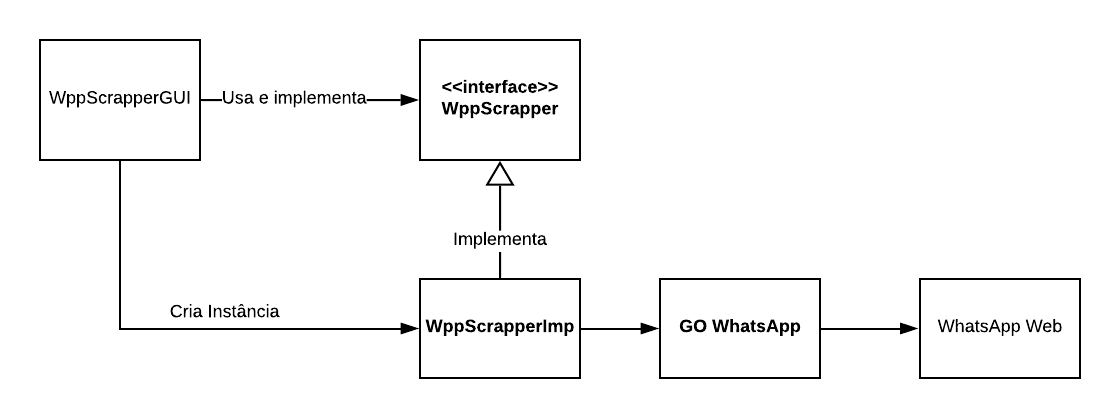
\includegraphics[width=\textwidth]{img/WppScrapperAPIs.png}
%     \caption{Diagrama de pacotes que demonstra como uma aplicação usuária da API \textit{WppScrapper}, exemplificada com o nome de \textit{WppScrapperGUI}, se relaciona com o \textit{WppScrapper} e sua implementação concreta, a \textit{WppScrapperImp}.}
%     \centering
%     \label{fig:WppScrapperAPIs}
% \end{figure}

Como visto anteriormente, a interface da \textit{WppScrapper} precisará ser sólida e agnóstica a detalhes de implementação interna. No diagrama da figura \ref{fig:WppScrapperClass} está ilustrado o que está aqui idealizado: o programa \textit{WppScrapperGUI} precisará referenciar a implementação concreta do \textit{WppScrapper} apenas no momento de criar a instância, diminuindo o impacto de mudanças internas. Tal como o \textit{WppScrapperGUI} o mesmo deve ser verdade para qualquer programa que use a API \textit{WppScrapper} para extrair mensagens trocadas por meio do WhatsApp.

\begin{figure}[!htb]
    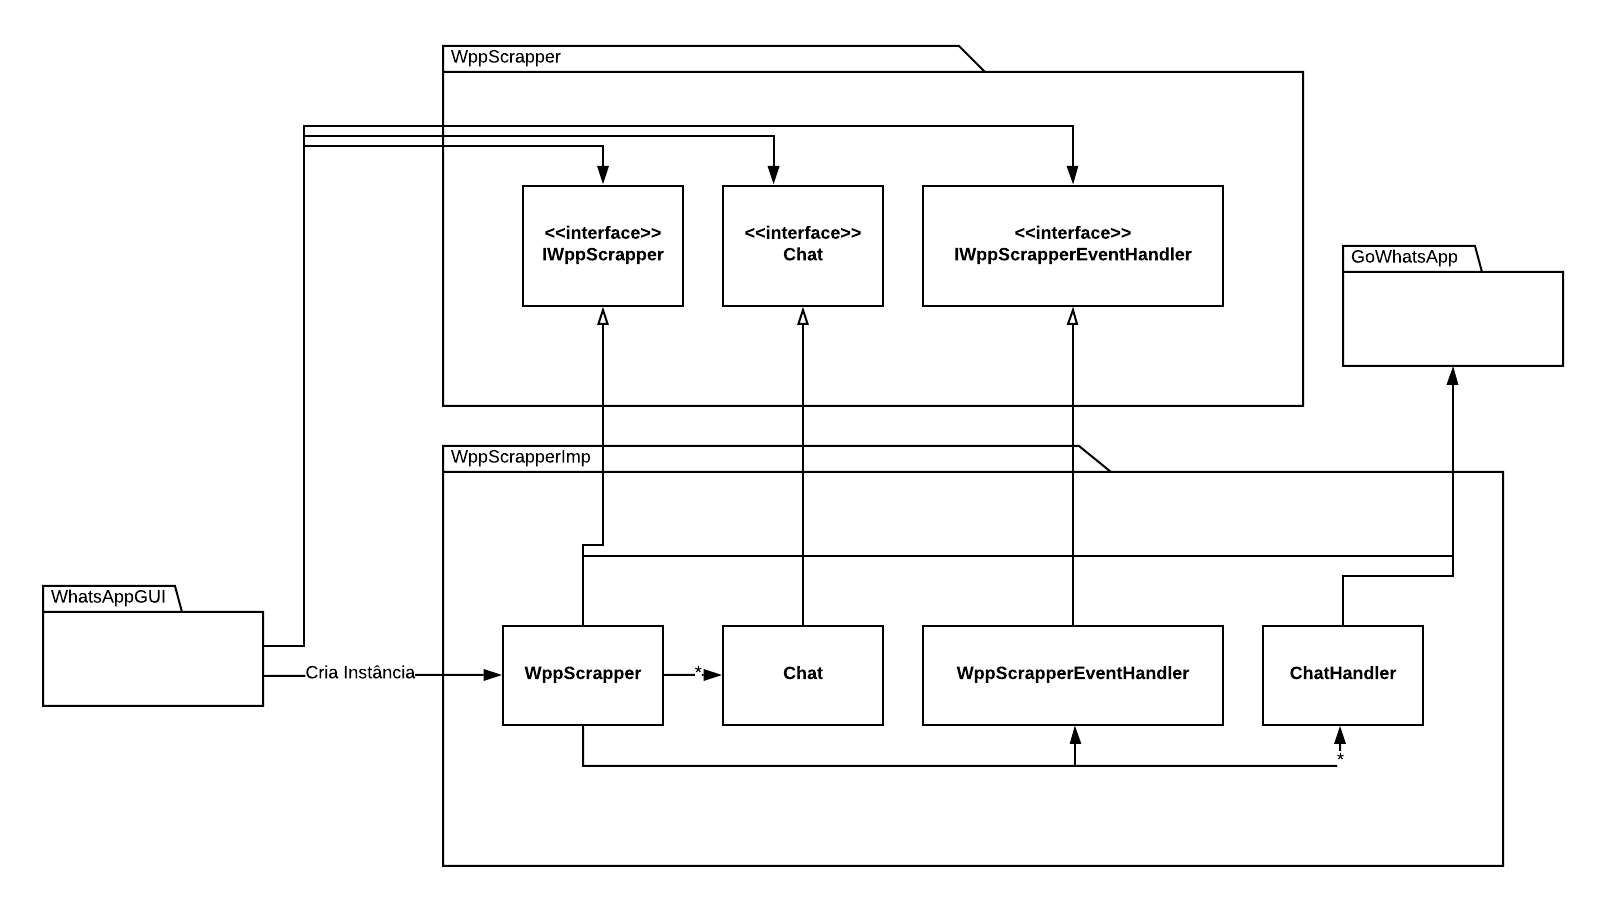
\includegraphics[width=\textwidth]{img/WppScrapperClass.png}
    \caption{Diagrama de pacotes simplificado com diagrama de classes simplificado que demonstra como o \textit{WppScrapper} se relaciona com o \textit{WppScrapperImp}, \textit{WppScrapperGUI} e com a API \textit{GoWhatsApp}.}
    \centering
    \label{fig:WppScrapperClass}
\end{figure}

A figura \ref{fig:WppScrapperInterfaces} descreve um diagrama de classes com a definição das interfaces de programação resultado de todos os requisitos descritos na  seção \ref{cap:proposta}. O usuário da API poderá instanciar uma implementação concreta da interface \textit{IWppScrapper} e através dela ter acesso às funcionalidades desejadas. Esse usuário também poderá implementar as interfaces que possuem sufixo \textit{Listener} e, usando a instância de \textit{IWppScrapperEventHandler} que é provida pela implementação de \textit{IWppScrapper} através da função \textit{GetAppScrapperEventHandler}, adicionar e remover \textit{Listeners} para receber os eventos desejados e poder responder a eles.

% \begin{tikzpicture} 
% \umlclass[type=interface, scale=0.7]{IWppScrapper}{
% }{
%  + Auth(qrChan chan <- string) (string, error) \\
%  + ReAuth(qrChan chan <- string, uuid string) (string, error) \\
%  + WaitInitialization() chan bool \\
%  + Initialized() bool \\
%  + GetChats() map[string]Chat \\
%  + StartScrapper(resume bool) \\
%  + StopScrapper() \\
%  + GetWppScrapperEventHandler() IWppScrapperEventHandler \\
% }
% \umlclass[type=interface, scale=0.7, x=-2,y=-6]{Chat}{
% }{
%  + Name() string \\
%  + Jid() string \\
%  + GetStatus() ChatStatus \\
% }

% \umlclass[type=interface, scale=0.7, x=5.5,y=-8]{IWppScrapperEventHandler}{
% }{
%     + AddOnScrapperStartedListenner(IWppScrapperStartedListener) \\
% 	+ AddOnScrapperStoppedListenner(IWppScrapperStoppedListener)\\
% 	+ AddOnScrapperFinishedListenner(IWppScrapperFinishedListener)\\
% 	+ AddOnChatScrapStartedListenner(IWppScrapperChatScrapStartedListener)\\
% 	+ AddOnChatScrapFinishedListenner(IWppScrapperChatScrapFinishedListener)\\

% 	+ RemoveOnScrapperStartedListenner(IWppScrapperStartedListener)\\
% 	+ RemoveOnScrapperStoppedListenner(IWppScrapperStoppedListener)\\
% 	+ RemoveOnScrapperFinishedListenner(IWppScrapperFinishedListener)\\
% 	+ RemoveOnChatScrapStartedListenner(IWppScrapperChatScrapStartedListener)\\
% 	+ RemoveOnChatScrapFinishedListenner(IWppScrapperChatScrapFinishedListener)\\
% }
% \umlclass[type=interface, scale=0.7, x=-1,y=-13]{IWppScrapperStartedListener}{
% }{
% 	OnWppScrapperStarted(wppScrapper IWppScrapper)

% }
% \umlclass[type=interface, scale=0.7, x=-1,y=-16]{IWppScrapperStoppedListener}{
% }{
% 	OnWppScrapperStopped(wppScrapper IWppScrapper)

% }
% \umlclass[type=interface, scale=0.7, x=-1,y=-19]{IWppScrapperFinishedListener}{
% }{
% 	OnWppScrapperFinished(wppScrapper IWppScrapper)

% }
% \umlclass[type=interface, scale=0.7, x=6,y=-13]{IWppScrapperChatScrapStartedListener}{
% }{
% 	OnWppScrapperChatScrapStarted(chat Chat)

% }
% \umlclass[type=interface, scale=0.7, x=6,y=-16]{IWppScrapperChatScrapFinishedListener}{
% }{
% 	OnWppScrapperChatScrapFinished(chat Chat)

% }
% \umluniassoc{IWppScrapper}{Chat}
% \umluniassoc{IWppScrapper}{IWppScrapperEventHandler}
% \umluniassoc{IWppScrapperEventHandler}{IWppScrapperChatScrapFinishedListener}
% \end{tikzpicture}

É de responsabilidade da implementação concreta implementar o \textit{IWppScrapperEventHandler} e disparar os eventos no momento correto. A implementação do \textit{WppScrapper} também possui a responsabilidade de implementar todas as outras funções de \textit{IWppScrapper} tal como uma função adicional para criar a instância da classe concreta que implementa tal interface. Na figura \ref{fig:WppScrapperClass} é possível identificar como as referências se dão. É possível ver que o módulo que contém as interfaces principais não possuem qualquer referência para fora do módulo e qualquer dependência da API \textit{GO WhatsApp} é isolada dentro da implementação concreta e pode ser substituída sem causar grandes impactos na interface ou nos usuários da API \textit{WppScrapper}.

\begin{figure}[!htb]
    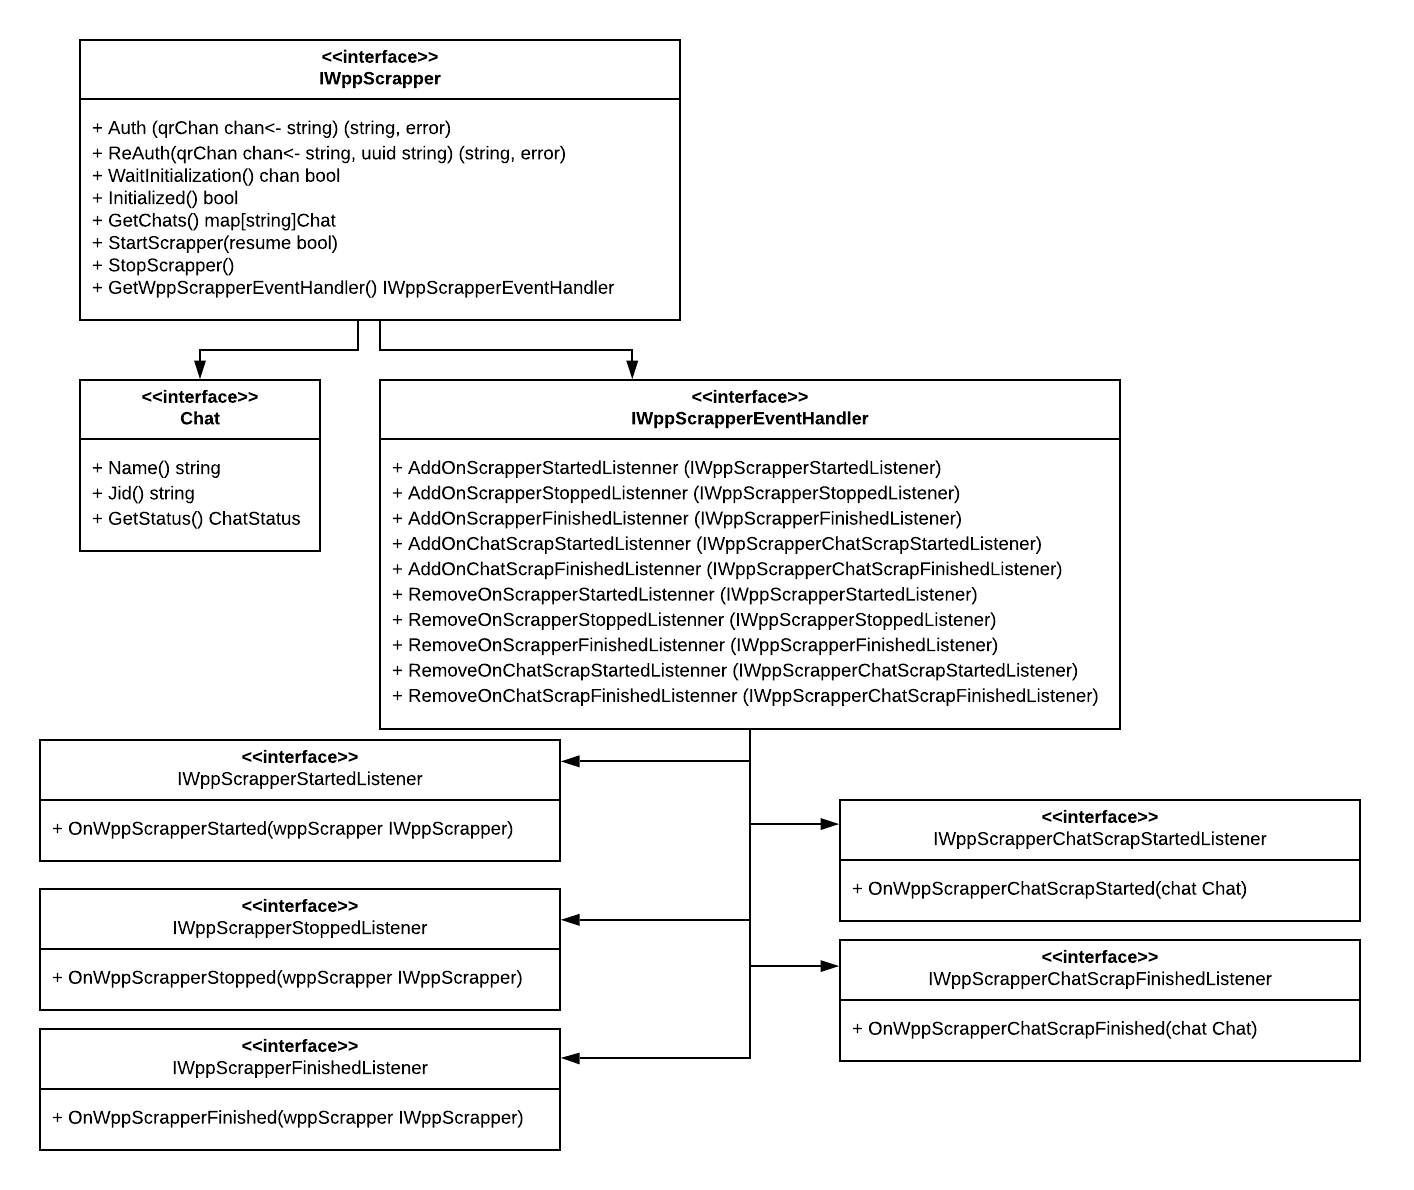
\includegraphics[width=\textwidth]{img/WppScrapperInterface.png}
    \caption{Diagrama de Classes com as interfaces que compõem o \textit{WppScrapper}}
    \centering
    \label{fig:WppScrapperInterfaces}
\end{figure}
Para que haja acesso às informações do WhatsApp, é necessária a autenticação com o uso do \textit{QRCode}. O \textit{WppScrapper} é capaz de recuperar esse \textit{QRCode} através da \textit{GO WhatsApp}. Como é possível ver no diagrama de sequência da figura \ref{fig:UML_Sequence_Auth}, onde está ilustrado o processo de autenticação, o programa recebe de forma assíncrona as informações do \textit{QRCode} e deve passar adiante para o usuário. Uma vez que o usuário realize o escaneamento do \textit{QRCode}, a função é capaz de retornar com sucesso. Não está ilustrado na figura, mas o usuário pode demorar mais que um tempo determinado; caso isso, ocorra a função irá retornar com erro de \textit{timeout}.

\begin{figure}[!htb]
    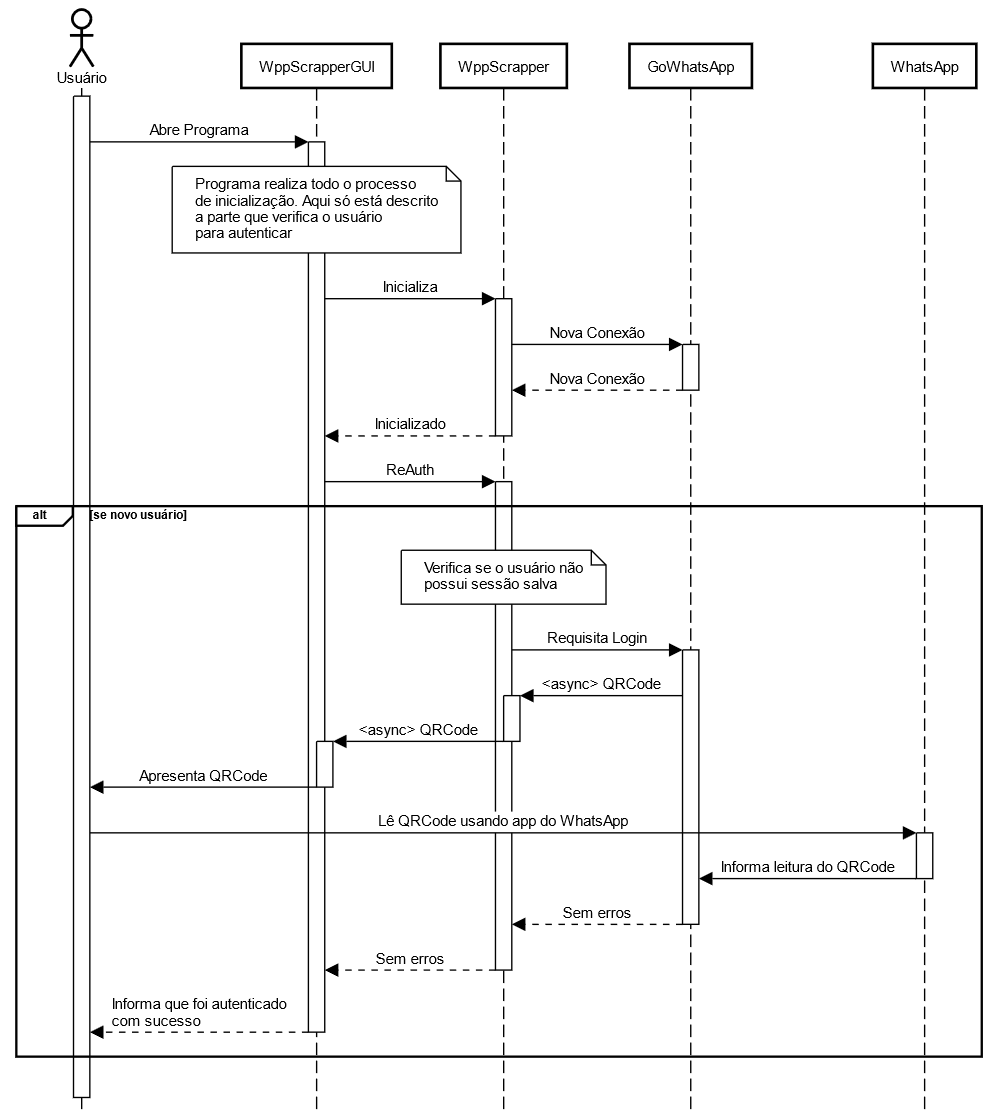
\includegraphics[width=\textwidth]{img/UML_Sequence_Auth.png}
    \caption{Diagrama da sequência que demonstra o processo de autenticação de um usuário sem sessão salva.}
    \centering
    \label{fig:UML_Sequence_Auth}
\end{figure}

Além das funções necessárias para que se requisite a execução de determinadas ações, como a autenticação (\textit{Auth}), inicialização da rotina de extração das mensagens (\textit{StartScrapper}), pausa dessa rotina (\textit{StopScrapper}) etc, o \textit{WppScrapper} também define uma série de eventos necessários para que a aplicação usuária possa responder adequadamente. Por exemplo, para saber quando a extração terminou, a aplicação usuária deverá implementar a interface \textit{IWppScrapperFinishedListerner} e registrar esse objeto junto ao objeto do tipo \textit{IWppScrapperEventHandler} provido pelo \textit{WppScrapper} através da função \textit{GetWppScrapperEventHandler}. Uma vez que esse objeto estiver registrado, ele terá a função \textit{OnWppScrapperFinished} chamada quando a extração foi concluída. A figura \ref{fig:UML_Sequence_EventAndStart} exemplifica esse processo. De maneira análoga, ocorre com os demais eventos, todos descritos no diagrama de classes da figura \ref{fig:WppScrapperInterfaces} com o sufixo \textit{Listener}.

% Para que a \textit{WppScrapperGUI} possa saber quando a extração das mensagens finalizou, ou quando a extração de alguma conversa específica terminou, dentre outros eventos, e poder responder a esses eventos de forma adequada, foi implementado uma série de eventos. Esses eventos podem ser escutados através das interfaces de sufixo Listener ilustradas na figura \ref{fig:WppScrapperInterfaces}. Na figura \ref{fig:UML_Sequence_EventAndStart} está ilustrado um diagrama de sequencia que exemplifica o processo de escutar o evento \textit{OnScrapperFinishedEvent}, que é disparado no momento em que o \textit{WppScrapper} finaliza de extrair todas as mensagens de todas as conversas.

\begin{figure}[h!]
    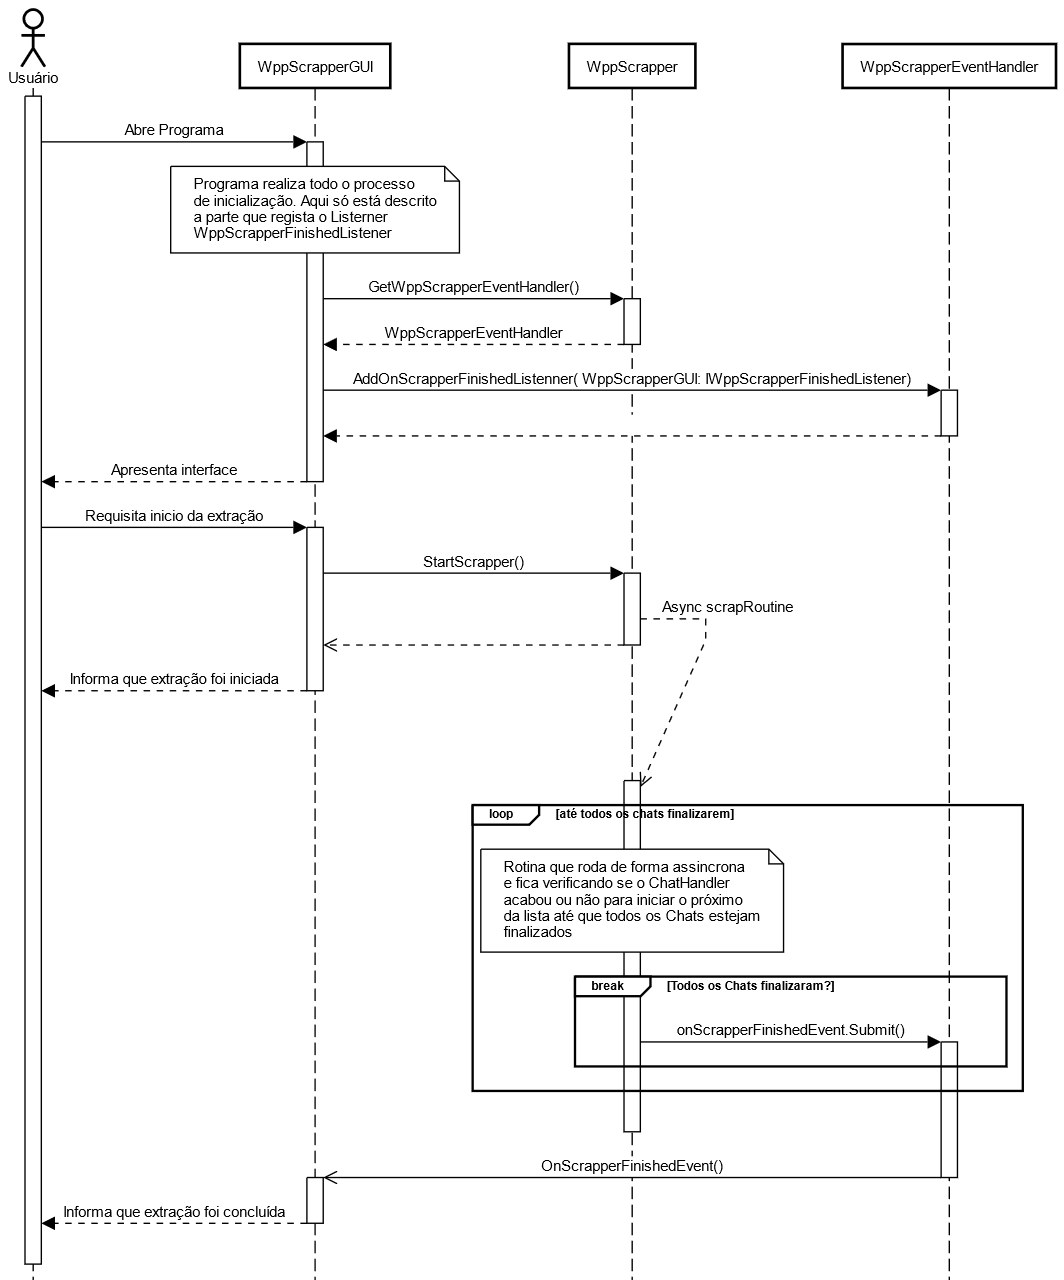
\includegraphics[width=\textwidth]{img/UML_Sequence_EventAndStart.png}
    \caption{Diagrama da sequência que demonstra o processo de registrar o \textit{Listerner} \textit{IWppScrapperFinishedListerner} até o momento que o mesmo é acionado.}
    \centering
    \label{fig:UML_Sequence_EventAndStart}
\end{figure}

Na próxima sessão, estará descrito o processo de implementação da \textit{WppScrapperGUI}. Junto a isso será possível encontrar mais exemplos de uso da \textit{WppScrapper}.

\section{Implementação da WppScrapperGUI}

Para realizar a implementação do \textit{WppScrapperGUI}, o primeiro desafio está na escolha de uma biblioteca de construção interface gráfica escrita na linguagem GO que atenda as necessidades. Ou seja, essa biblioteca deveria permitir que o programa resultante seja executado nos diferentes sistemas operacionais, (\textit{e.g.} \textit{Windows}, \textit{Linux}), que seja estável, tenha uma interface de programação bem documentada e estruturada, possua o conjunto de funcionalidades e elementos visuais e interativos necessários, (\textit{e.g Botão, Texto, Tabela, Imagem}) e que a interface gráfica gerada por ela seja agradável aos olhos do usuário.

Dentre as bibliotecas estudadas e testadas, aquela se mostrou melhor para atender as necessidades do projeto foi a \textit{Fyne.io}\footnote{https://fyne.io/}. A facilidade para gerar os programas executáveis para diferentes plataformas, a simplicidade da biblioteca de construção da interface gráfica, boa documentação, o \textit{design} padrão aceitável da interface gerada e ser de código aberto foram as características que foram decisivas para que tenha sido a escolhida.

Para atender aos requisitos definidos no capítulo \ref{cap:proposta}, a interface de usuário implementa duas telas. A primeira é a tela de autenticação, onde o QRCode é apresentado para o usuário e a segunda tela é onde, uma vez autenticado, o usuário poderá iniciar a extração das mensagens. O \textit{WppScrapperGUI} ainda apresenta uma terceira tela de carregamento. Nela não é possível nenhuma interação e é apresentada enquanto alguma operação de transição entre as telas está sendo realizada.

Na figura \ref{fig:Code_Main_Func} está apresentado o trecho do código responsável pela iniciação do programa. É iniciado como variáveis globais as referências às partes principais da biblioteca do \textit{Fyne.io}, pelas quais será possível alterar o conteúdo da janela visível ao usuário, e com uma referência a uma instância do \textit{IWppScrapper}, que foi explicado no capitulo \ref{cap:wppscrapper}. Na função \textit{main} é configurado o tamanho da janela e então chamado a função \textit{ShowAndRun} do \textit{Fyne.io}, que é quando uma janela é aberta, apresentada ao usuário e toda a biblioteca do \textit{Fyne.io} passa a ser executada.

\begin{figure}[h!]
    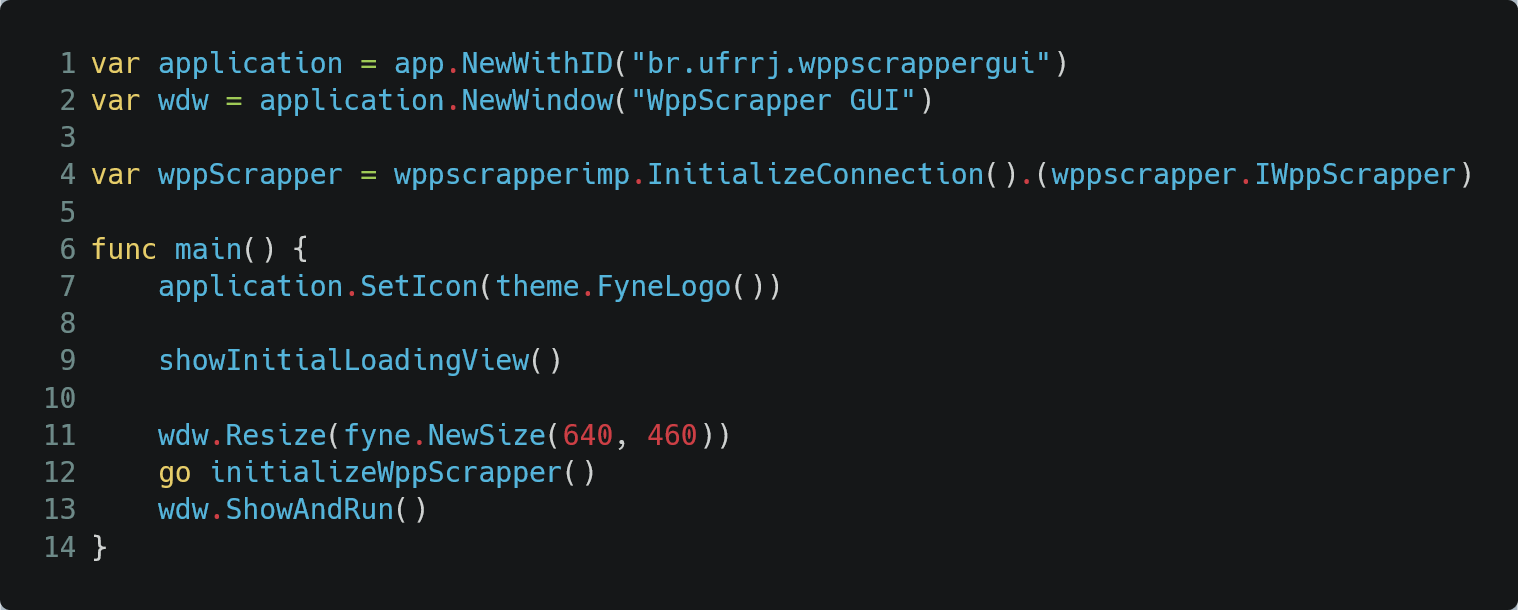
\includegraphics[width=\textwidth]{img/code_main_func.png}
    \caption{Trecho de inicialização do \textit{WppScrapperGUI}.}
    \centering
    \label{fig:Code_Main_Func}
\end{figure}

Ainda na figura \ref{fig:Code_Main_Func} é possível ver que há a chamada da função \textit{showInitialLoadingView}. Essa função somente apresenta na janela um texto informando ao usuário que o programa está carregando. Nesse mesmo trecho de código tem a chamada assíncrona para função \textit{initializeWppScrapper}, que está inteiramente ilustrada na figura \ref{fig:initializeWppScrapper}. Essa função é responsável por requisitar o \textit{QRCode} para o \textit{WppScrapper} e então passá-lo para a função que irá apresentá-lo na janela. Essa função está ilustrada na figura \ref{fig:code_showQrCodeView} e a janela resultado da função na figura \ref{fig:gui_qrCode}. A função ainda trata que, caso ocorra algum erro, ela será chamada novamente de forma recursiva para que um novo \textit{QRCode} seja requisitado apresentado ao usuário. 

Caso não ocorra erros, ou seja, o usuário realize a leitura do \textit{QRCode} corretamente, é apresentado ao usuário a janela de \textit{carregando} novamente enquanto o WppScrapper não termina de inicializar. Uma vez inicializado, o programa chama a função \textit{showMainView}, que é responsável por requisitar a apresentação da segunda tela, a tela onde é possível iniciar a extração das mensagens.

\begin{figure}[h!]
    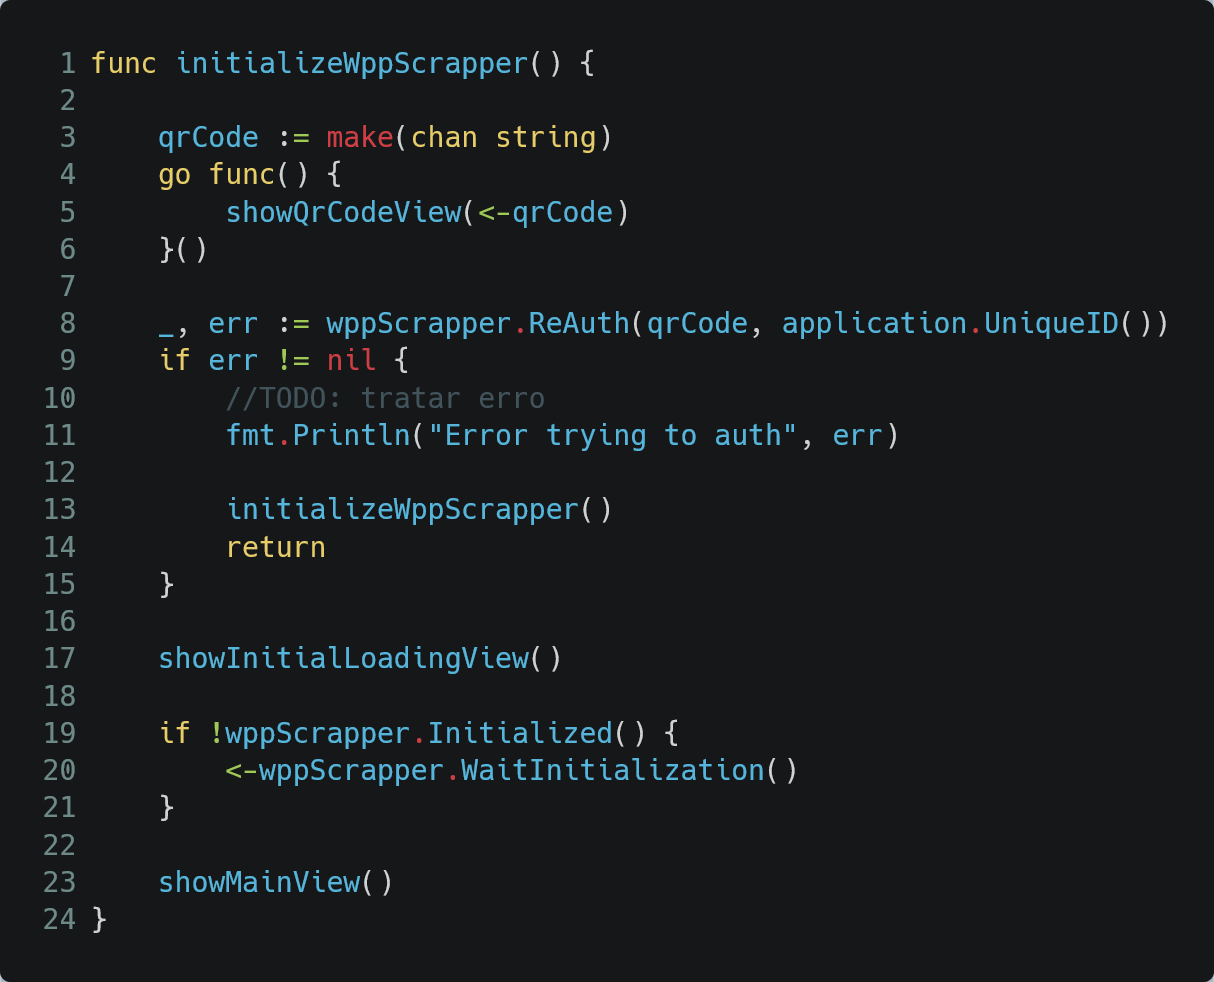
\includegraphics[width=\textwidth]{img/code_initializeWppScrapper.png}
    \caption{Trecho de código que trata a autenticação do usuário.}
    \centering
    \label{fig:initializeWppScrapper}
\end{figure}

\begin{figure}[h!]
    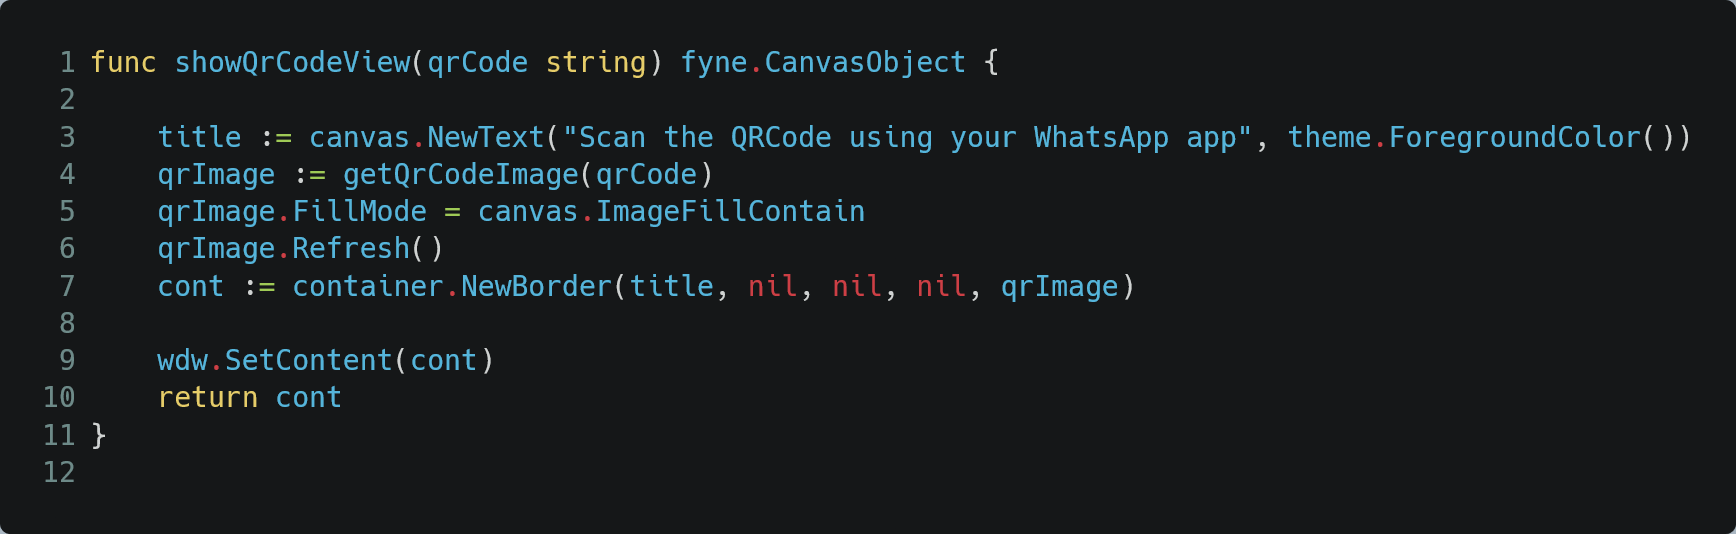
\includegraphics[width=\textwidth]{img/code_showQrCodeView.png}
    \caption{Trecho de código que apresenta o QRCode ao usuário.}
    \centering
    \label{fig:code_showQrCodeView}
\end{figure}

\begin{figure}[h!]
    \centering
    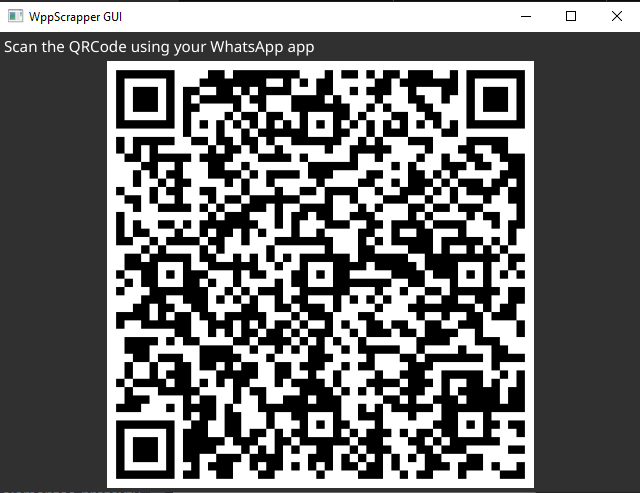
\includegraphics[width=0.5\textwidth]{img/gui_qrCode.png}
    \caption{Janela que apresenta o QRCode ao usuário.}
    \label{fig:gui_qrCode}
\end{figure}

A função \textit{showMainView} apenas cria uma nova instancia do tipo \textit{MainView} e requisita que a mesma apresente seu conteúdo através da função \textit{Show}. Esse tipo é responsável por construir a tela que permite ao usuário iniciar a extração do conteúdo, pausar a mesma e recomeçar, caso deseje. Nessa janela o usuário também tem acesso ao estado atual do programa, \textit{e.g.} executando a extração, esperando, finalizado, tal como informação do estado de cada \textit{Chat}.

Nessa parte do programa é possível encontrar bons exemplos de uso da API \textit{WppScrapper}. Na função \textit{buildHeader}, parcialmente apresentada na figura \ref{fig:code_buildHeader_btns}, é possível ver o código executado quando os botões são acionados pelo usuário. Já na figura \ref{fig:code_listeners} encontramos exemplo de código que implementa os listeners definidos na API \textit{WppScrapper} e usa a mesma API para assinar a instancia e passar a 'escutar' caso algum desses eventos ocorra. Assim o programa pode responder e esconder determinados botões a depender do estado do programa, como por exemplo esconde os botões que iniciam a extração das mensagens quando o programa já está extraindo as mensagens e apresentar apenas o botão que pausa essa execução.

\begin{figure}[h!]
    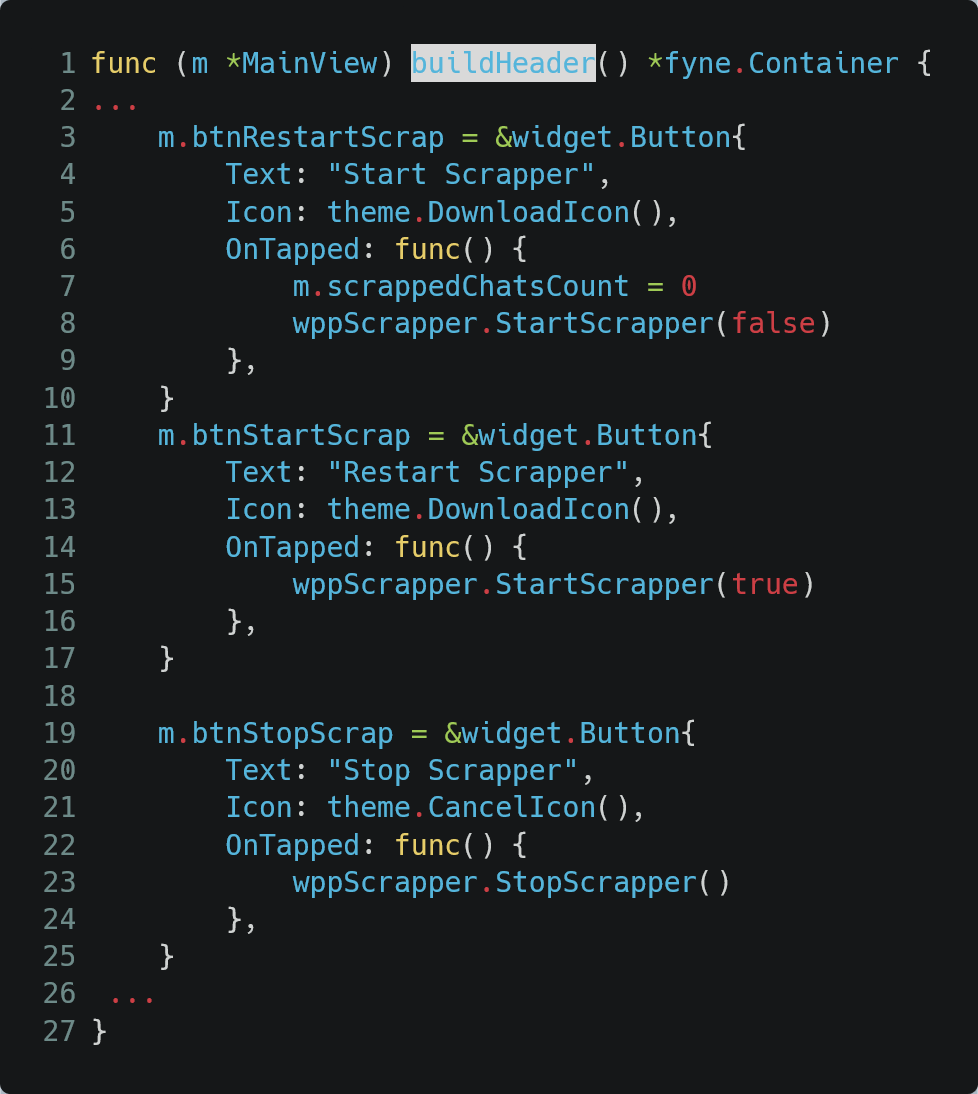
\includegraphics[width=\textwidth]{img/code_buildHeader_btns.png}
    \caption{Parte da função \textit{buildHeader} do tipo \textit{MainView} que cria os botões que inicia a extração, pausa a mesma e reinicia. Parte da função foi omitida.}
    \centering
    \label{fig:code_buildHeader_btns}
\end{figure}

\begin{figure}[h!]
    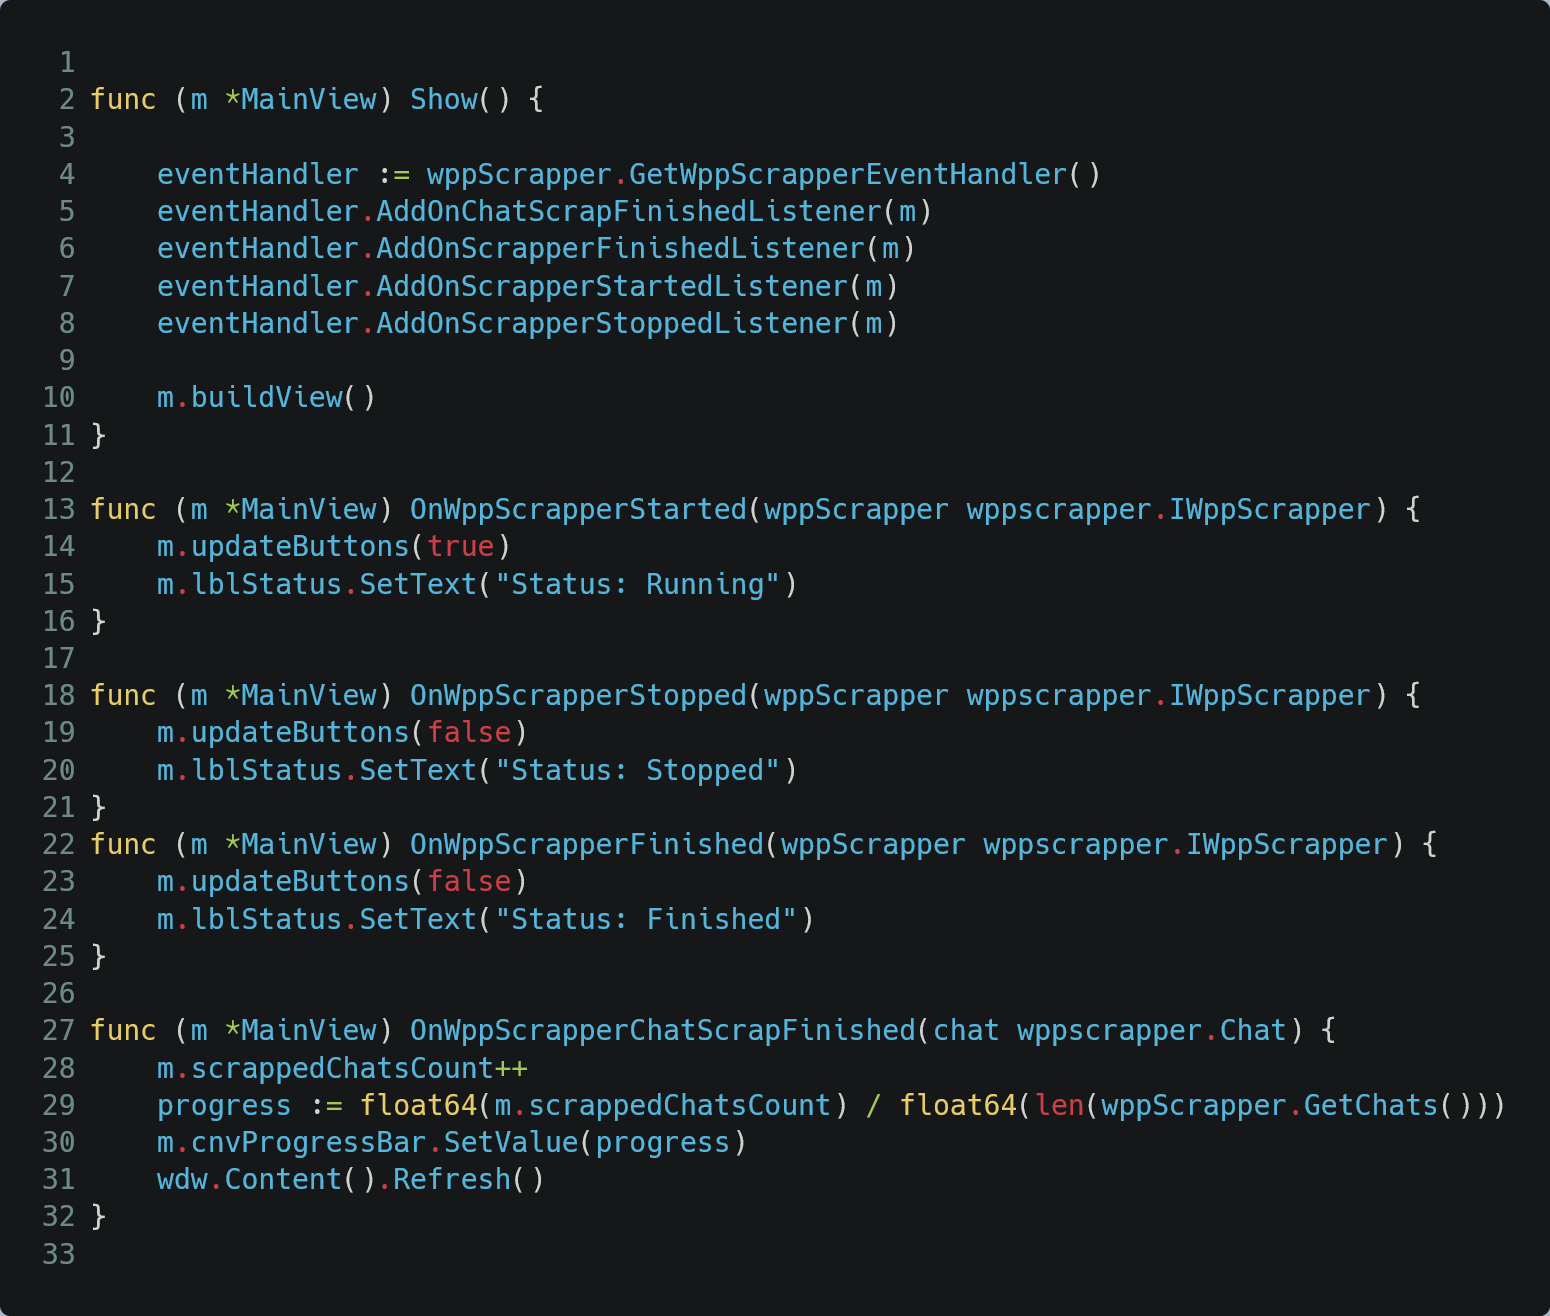
\includegraphics[width=\textwidth]{img/code_listeners.png}
    \caption{Trecho de código que define funções para o tipo \textit{MainView}. Nesse trecho é possível encontrar a implementação das interfaces da API \textit{WppScrapper}.}
    \centering
    \label{fig:code_listeners}
\end{figure}


% Objetivo é implementar uma iterface visual. Não há tantas preocupações arquiteturais pois é um sistema simples onde a logica de negócio ja está implementada no WppScrapper

% Dentre as opções de bibliotecas de interface grafica disponíveis para GO, foi escolhido o Fyne devido a sua facilidade e simplicidade. As possibilidades de customização são limitadas, mas ja ter uma sorte de elementos prontos para uso e de aparencia aceitável é um bom diferencial.

% Alem disso o fyne mantém a possibilidade de realização de build para muiltiplas plataformas do go, disponibilizando uma ferramenta que possibilita contruir aplicação para linux, windows ou osx facilmente de qualquer máquina, bastando essa possuir o go e o docker instalado.

% Uma vez decido a api de interface gráfica, bastava implementar o código que gerava a interface e conectava com o WppScrapper, seja respondendo as mudanças de estado do scrapper quanto realizando chamadas no mesmo.


\section{Demonstração do WppScrapperGUI}

Com intuito de realizar uma pequena demonstração do \textit{WppScrapperGUI} em ação, essa secção descreve um procedimento bastante simplificado de coleta de mensagens de grupos públicos de WhatsApp. Os \textit{links} para acesso aos grupos foram encontrados disponíveis no \textit{Google} e no \textit{Facebook}. Para a realização da operação, foi utilizada uma conta de WhatsApp criada apenas para essa finalidade.

O primeiro passo realizado foi a inscrição dessa conta nos grupos públicos. Como a intenção era realizar apenas uma pequena amostra, foi feita a inscrição em 10 grupos de temas variados, \textit{e.g.} futebol, jogos. As inscrições foram feitas às 20h de um dia e deixou-se coletando as mensagens até às 13h do dia seguinte, quando foi feito o uso do \textit{WppScrapperGUI} para realizar a extração das mensagens. 

Nas figuras \ref{fig:wppscrapper-idle}, \ref{fig:wppscrapper-running2} e \ref{fig:wppscrapper-finished} encontra-se exemplo do programa aberto em seus três diferentes estados. No primeiro o programa acabara de ser aberto e tem listado todas as conversas encontradas em estado de espera, apresentado na figura \ref{fig:wppscrapper-idle}. Em seguida, após acionado pelo usuário a realizar a extração, o programa modifica parte da sua interface para indicar seu estado, apresentar as opções de ação possível e indicar a conversa que está sendo extraído no momento, tal como seu indicador de progresso passa a indicar uma porcentagem referente a quantidade de conversas extraídas frente ao total de conversas a se extrair, ilustrado na figura \ref{fig:wppscrapper-running2}. Por ultimo o programa apresenta a tela de finalizado, onde todas as conversas já foram extraídas e se encontram em formato CSV no computador do usuário na mesma pasta em que se encontra o executável do programa, ilustrado na figura \ref{fig:wppscrapper-finished}.

\begin{figure}[!htb]
    \centering
    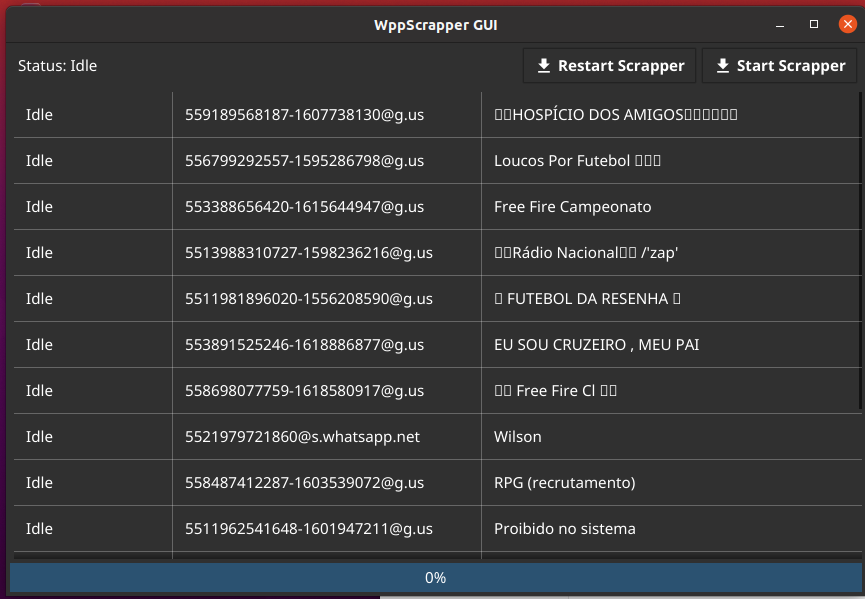
\includegraphics[width=0.8\textwidth]{img/wppscrapper-idle.png}
    \caption{Captura de tela do \textit{WppScrapperGUI} em estado de espera logo após de ter o usuário validado e carregar todas as informações.}
    \label{fig:wppscrapper-idle}
\end{figure}

\begin{figure}[!htb]
    \centering
    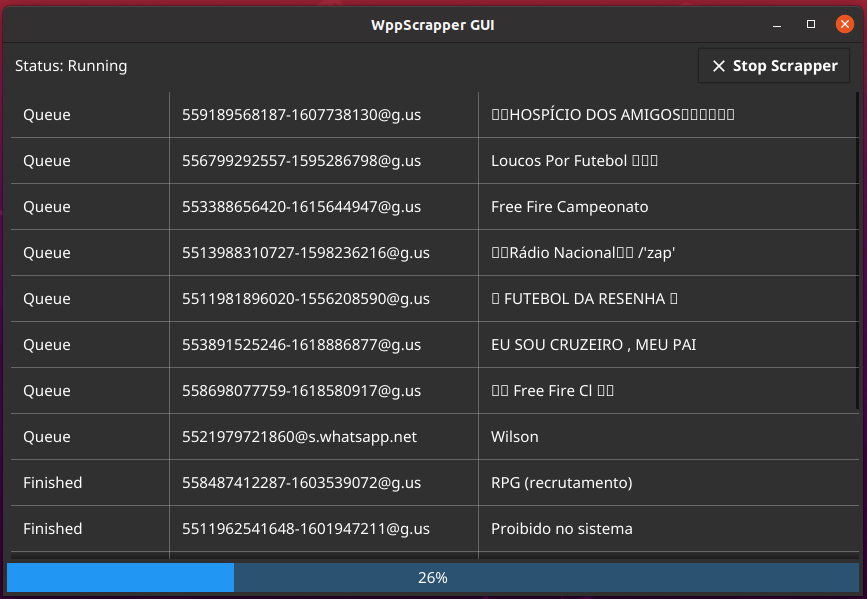
\includegraphics[width=0.8\textwidth]{img/wppscrapper-running2.png}
    \caption{Captura de tela do \textit{WppScrapperGUI} rodando a rotina de extração das mensagens, onde $26\%$ das conversas já foram extraídas.}
    \label{fig:wppscrapper-running2}
\end{figure}

\begin{figure}[!htb]
    \centering
    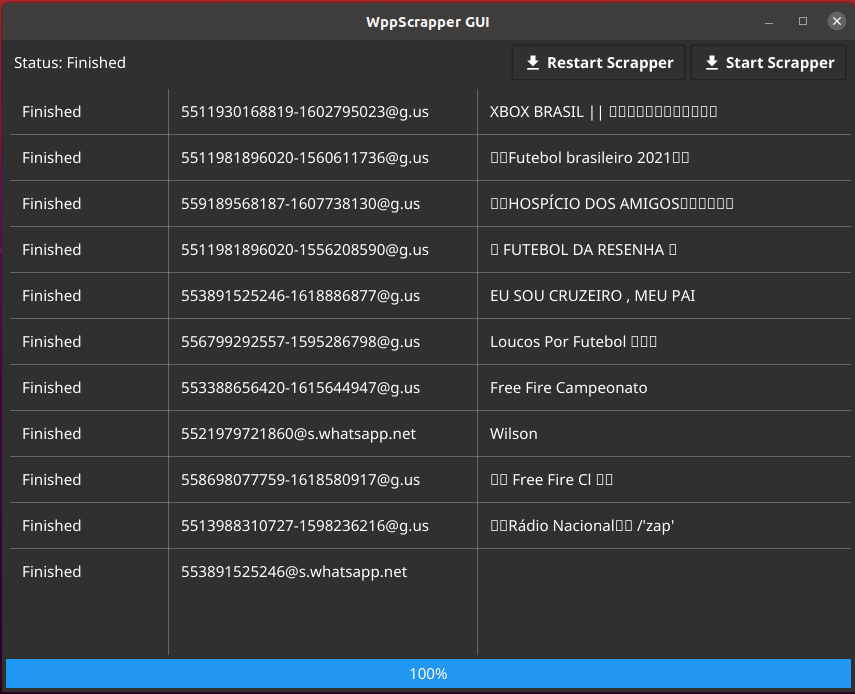
\includegraphics[width=0.8\textwidth]{img/wppscrapper-finished.png}
    \caption{Captura de tela do \textit{WppScrapperGUI} após finalizar de extrair todas as conversas.}
    \label{fig:wppscrapper-finished}
\end{figure}

Neste exemplo, foi possível coletar e extrair um total de 1472 mensagens de 10 diferentes grupos que possuem, no total, 1311 usuários não necessariamente distintos. Na tabela \ref{fig:result} é possível encontrar esses dados descritos para cada grupo tal como seu nome.

% \begin{figure}[!htb]
%     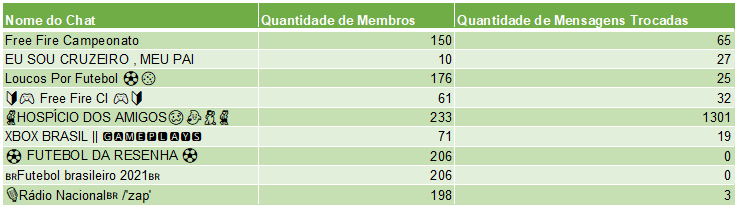
\includegraphics[width=\textwidth]{img/result_extract.png}
%     \caption{Trecho de código que define funções para o tipo \textit{MainView}. Nesse trecho é possível encontrar a implementação das interfaces da API \textit{WppScrapper}.}
%     \centering
%     \label{fig:result}
% \end{figure}


\begin{table}[!htb]
  \centering
  \caption{Tabela de nome dos grupos que tiveram mensagens extraídas com a quantidade de membros e a quantidade de mensagens extraídas por grupo.}
    \label{fig:result}
%   \rowcolors{1}{light-gray}
  \begin{tabular}{l c c c}
  \toprule
    Nome do Chat & Quantidade de Membros & Quantidade de Mensagens \\
    \midrule
        Free Fire Campeonato & 150 & 65  \\
        
        EU SOU CRUZEIRO , MEU PAI & 10 & 27  \\
        
        Loucos Por Futebol & 176 & 25  \\
        
        Free Fire Cl & 61 & 32  \\
        
        HOSPÍCIO DOS AMIGOS & 233 & 1301  \\
        
        XBOX BRASIL & 71 & 19  \\
        
        FUTEBOL DA RESENHA & 206 & 0  \\
        
        Futebol brasileiro 2021 & 206 & 0  \\
        
        Rádio Nacional & 198 & 3  \\
    \bottomrule
  \end{tabular}
\end{table}

A seguir temos exemplos de arquivos extraídos, em todas as imagens os identificadores, que possuem o número de celular em sua composição, foram borrados para preservar privacidade daqueles que enviaram as mensagens e que participam do grupo em questão. Na figura \ref{fig:csv-msgs} é possível observar, entre outras informações, as mensagens enviadas no grupo "Free Fire Campeonato". Com dados do mesmo grupo, na figura \ref{fig:csv-group} está ilustrado as informações do grupo em si, como o identificador do seu criador e a descrição do grupo. O arquivo com os membros deste grupo está ilustrado na imagem \ref{fig:csv-msgs}. 

\begin{figure}[!htb]
    \centering
    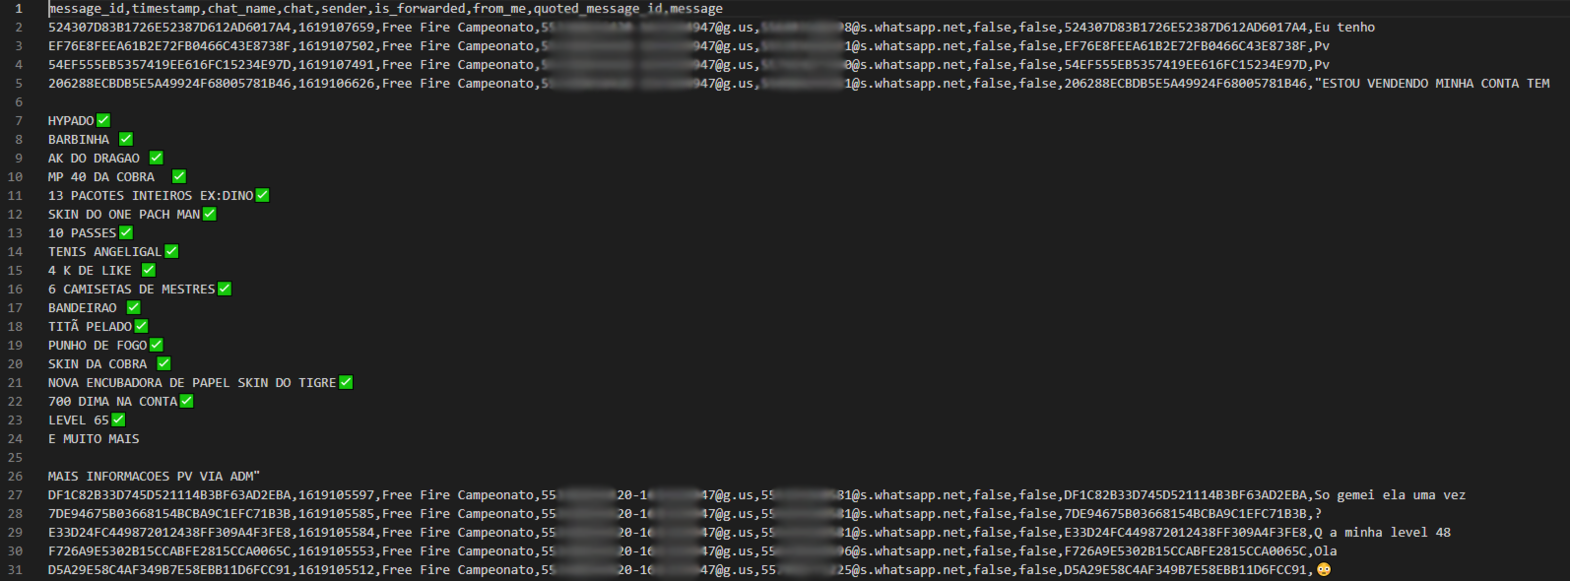
\includegraphics[width=1\textwidth]{img/csv_msgs.png}
    \caption{Captura de tela da parte inicial do conteúdo de um arquivo CSV de mensagens gerado pela extração.}
    \label{fig:csv-msgs}
\end{figure}

\begin{figure}[!htb]
    \centering
    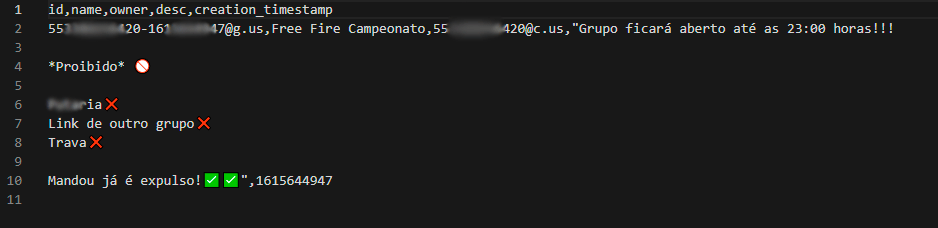
\includegraphics[width=1\textwidth]{img/csv_group.png}
    \caption{Captura de tela do conteúdo um arquivo \textit{CSV} de descrição de um grupo gerado pela extração.}
    \label{fig:csv-group}
\end{figure}

\begin{figure}[!htb]
    \centering
    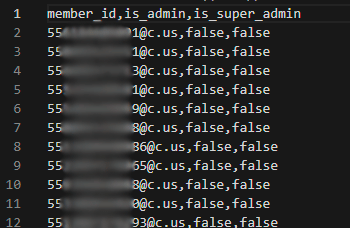
\includegraphics[width=0.7\textwidth]{img/csv_members.png}
    \caption{Captura de tela da parte inicial do conteúdo um arquivo \textit{CSV} de lista de membros de um grupo gerado pela extração.}
    \label{fig:csv-members}
\end{figure}


% \begin{table}[!htb]
% \centering
% \caption{Lista dos parâmetros e seus respectivos valores para cada modelo que será otimizado através do algoritmo genético.}
% \begin{tabular}{llc}
% \toprule
% Modelo                       & Parâmetro                 & Valores \\
% \midrule
% \multirow{6}{*}{Rede Neural} & Variáveis Latentes        & $\{x \mid x = 10 + 10 \cdot i  , 0 \leq  i \leq 9 \} \cup \{150\}$ \\ %[10:10:100..., 150]
%                              & Neurônios                 & $\{x \mid x = 100 + 50 \cdot i  , 0 \leq  i \leq 8 \}$ \\ %[100:50:500...]
%                              & Dropout                   & $\{x \mid x = 0.1 \cdot i  , 0 \leq  i \leq 10 \}$ \\ %[0:0.1:1...]
%                              & Batch                     & $\{64, 128, 256\}$ \\ % [64, 128, 256]
%                              & Épocas                    & $\{10, 20, 30, 50\}$ \\ %[10, 20, 30, 50]
%                              & Paciência                 & $\{1, 2, 3, 4, 5\}$ \\ \midrule %[1, 2, 3, 4, 5]
% IRSVD                        & Variáveis Latentes        & $\{1, 2\} \cup \{x \mid x = 10 \cdot i  , 1 \leq  i \leq 9 \}$ \\ %[1 2 10:10:100...]
%                              & Taxa de Aprendizagem      & $\{x \mid x = 0.01 \cdot i  , 0 \leq  i \leq 10 \}$ \\ % [0:0.01:0.1...]
%                              & Regularização             & $\{x \mid x = 0.01 \cdot i  , 0 \leq  i \leq 10 \}$ \\ \midrule %[0:0.01:0.1...]
% KNN                          & Número Mínimo de Vizinhos & $\{5, 10\}$  \\ %[5 10]
%                              & Número de Vizinhos        & $\{15, 30, 50\}$ \\ %[15 30 50]
% \bottomrule
% \end{tabular}
% \label{tab:gaparam}
% \end{table}
\chapter{Conclusão}

Estudar como se dá as interações entre os usuários do WhatsApp\footnote{www.whatsapp.com} se tornou uma ferramenta poderosa para que pesquisadores e jornalistas possam melhor compreender os eventos da sociedade. Apesar de o aplicativo de mensagens instantânea não disponibilizar nenhuma ferramenta ou \textit{API} para que essas pessoas possam realizar seus estudos, o presente trabalho apresentou uma alternativa que pode ser usada.

No presente trabalho foi apresentado duas ferramentas, a API WppScrapper e a aplicação de interface gráfica para essa API chamada WppScrapperGUI. A aplicação se mostrou capaz de realizar a extração de mensagens de uma conta do WhatsApp, o que pode ser considerada uma tarefa essencial para realização de novos trabalhos acadêmicos que objetivem compreender essas mensagens. Se diferenciando de outras alternativas disponíveis, a aplicação possui uma interface gráfica, o que a torna mais acessível. 

Enquanto outras ferramentas similares necessitam de conhecimentos de programação para instalar e utilizar, a aplicação apresentada nesse trabalho consegue ser usada apenas executando um arquivo binário que pode ser baixado e sua operação pode ser realizada inteiramente através de uma interface gráfica. A disponibilização da \textit{API} WppScapper, que é análoga, porém agnóstica, a interface gráfica pode possibilitar que pesquisadores com conhecimento de programação a sua utilização em computadores remotos ou até a criação de novas formas de interface, \textit{e.g.} \textit{WebSocket}, \textit{REST}, \textit{CLI} etc.

Apesar de útil para coletar as mensagens textuais do WhatsApp, ambas as ferramentas apresentadas são limitadas e incapazes de coletar as imagens, mensagens de áudio ou de vídeo do WhatsApp. As ferramentas também não são capazes de extrair outras informações que podem ser úteis, \textit{e.g.}  imagem do grupo, foto de usuários. 

Para trabalhos futuros, além de implementar melhorias na aplicação para que essas limitações não estejam mais presentes, seria interessante realização de estudos, que utilize das mensagens extraídas e de técnicas de mineração de texto, com o objetivo de extrair informações relevantes, \textit{e.g} as tendências mais comentadas dentro dos grupos públicos de um determinado tópico.

Outras melhorias ainda podem ser feitas, no futuro, na aplicação e na API. A possibilidade de configurar um serviço armazenamento em nuvem, \textit{e.g.} \textit{Amazon S3}\footnote{https://aws.amazon.com/pt/s3/}, para armazenar os arquivos gerados pela extração, pode ser uma funcionalidade interessante, tal como a possibilidade de instalar a ferramenta em uma hospedagem remota, podendo proporcionar mais velocidade e disponibilidade. A possibilidade de extrair as mensagens em outros formatos, ( \textit{e.g.} \textit{Json}\footnote{https://json.org/json-pt.html}) também pode ser desejada.

Tanto o \textit{WppScrapper}\footnote{https://github.com/ribeiroferreiralucas/wpp-scrapper} quanto o \textit{WppScrapperGUI}\footnote{https://github.com/ribeiroferreiralucas/wpp-scrapper-gui} estão disponíveis no \textit{Github} em código aberto e contribuições são muito bem vindas. A melhoria das práticas de integração e entrega contínua, já parcialmente implementadas fazendo uso do \textit{Github Actions}\footnote{https://github.com/features/actions}, ou adição de testes unitários em ambas as ferramentas são apenas alguns exemplos de contribuições. Outros tipos de contribuição partindo de necessidades específicas de cada uso futuro também podem ser propostas e incorporadas ao código fonte.

Existe uma infinidade de estudos que podem ser feitos utilizando os dados possíveis de serem extraídos da aplicação aqui apresentada e muitas melhorias possíveis de serem feitas nela. O presente trabalho espera ter contribuído para que mais pesquisadores possam, além de contribuir com a evolução dessa ferramenta, esclarecer mais o que acontece no ambiente interno da rede social e que a sociedade possa fazer bom uso de tal poder.
% \input{elementos-textuais/topico-4}
% \input{elementos-textuais/topico-5}
\pagebreak

% BIBLIOGRAFIA
\makebibspage{elementos-postextuais/referencias}

% APÊNDICE

%\appendix
%\chapter{Lorem ipsum dolor sit amet}\label{chp:LABEL_APP_1}

Lorem ipsum dolor sit amet, consectetur adipiscing elit. Donec lacus nisl, ultricies vitae semper eu, scelerisque nec enim. Curabitur posuere tortor orci, at porta leo laoreet et. Quisque ut congue dolor. Maecenas vel sagittis diam. Praesent fermentum eleifend mi, sit amet vehicula leo pellentesque quis. Curabitur mattis luctus pulvinar. Proin auctor est nec nulla pellentesque commodo. Donec nec justo eu magna aliquet eleifend. Curabitur tristique tortor id sem dignissim, a iaculis metus interdum. Phasellus bibendum velit sit amet interdum semper. Nam vestibulum dui quis nisi consectetur, id vehicula dolor faucibus.

\end{document}